
%% bare_jrnl.tex
%% V1.4b
%% 2015/08/26
%% by Michael Shell
%% see http://www.michaelshell.org/
%% for current contact information.
%%
%% This is a skeleton file demonstrating the use of IEEEtran.cls
%% (requires IEEEtran.cls version 1.8b or later) with an IEEE
%% journal paper.
%%
%% Support sites:
%% http://www.michaelshell.org/tex/ieeetran/
%% http://www.ctan.org/pkg/ieeetran
%% and
%% http://www.ieee.org/

%%*************************************************************************
%% Legal Notice:
%% This code is offered as-is without any warranty either expressed or
%% implied; without even the implied warranty of MERCHANTABILITY or
%% FITNESS FOR A PARTICULAR PURPOSE! 
%% User assumes all risk.
%% In no event shall the IEEE or any contributor to this code be liable for
%% any damages or losses, including, but not limited to, incidental,
%% consequential, or any other damages, resulting from the use or misuse
%% of any information contained here.
%%
%% All comments are the opinions of their respective authors and are not
%% necessarily endorsed by the IEEE.
%%
%% This work is distributed under the LaTeX Project Public License (LPPL)
%% ( http://www.latex-project.org/ ) version 1.3, and may be freely used,
%% distributed and modified. A copy of the LPPL, version 1.3, is included
%% in the base LaTeX documentation of all distributions of LaTeX released
%% 2003/12/01 or later.
%% Retain all contribution notices and credits.
%% ** Modified files should be clearly indicated as such, including  **
%% ** renaming them and changing author support contact information. **
%%*************************************************************************


% *** Authors should verify (and, if needed, correct) their LaTeX system  ***
% *** with the testflow diagnostic prior to trusting their LaTeX platform ***
% *** with production work. The IEEE's font choices and paper sizes can   ***
% *** trigger bugs that do not appear when using other class files.       ***                          ***
% The testflow support page is at:
% http://www.michaelshell.org/tex/testflow/



\documentclass[journal]{IEEEtran}
%
% If IEEEtran.cls has not been installed into the LaTeX system files,
% manually specify the path to it like:
% \documentclass[journal]{../sty/IEEEtran}





% Some very useful LaTeX packages include:
% (uncomment the ones you want to load)


% *** MISC UTILITY PACKAGES ***
%
%\usepackage{ifpdf}
% Heiko Oberdiek's ifpdf.sty is very useful if you need conditional
% compilation based on whether the output is pdf or dvi.
% usage:
% \ifpdf
%   % pdf code
% \else
%   % dvi code
% \fi
% The latest version of ifpdf.sty can be obtained from:
% http://www.ctan.org/pkg/ifpdf
% Also, note that IEEEtran.cls V1.7 and later provides a builtin
% \ifCLASSINFOpdf conditional that works the same way.
% When switching from latex to pdflatex and vice-versa, the compiler may
% have to be run twice to clear warning/error messages.

\usepackage{booktabs}  % professionally typeset tables
\usepackage{amsmath}%,amssymb,amsfonts}
\usepackage{textcomp}  % better copyright sign, among other things
\usepackage{mathtools}% http://ctan.org/pkg/mathtools
\usepackage[binary-units=true]{siunitx}

%\usepackage{xcolor}
\usepackage{lipsum}    % filler text

\usepackage{outlines} % for bullets
\usepackage[%
%    font={small,sf},
%   labelfont=bf,
    format=hang,    
    format=plain,
    margin=0pt,
    width=0.8\textwidth,
]{caption}
\usepackage[list=true]{subcaption}






% *** CITATION PACKAGES ***
%
%\usepackage{cite}
% cite.sty was written by Donald Arseneau
% V1.6 and later of IEEEtran pre-defines the format of the cite.sty package
% \cite{} output to follow that of the IEEE. Loading the cite package will
% result in citation numbers being automatically sorted and properly
% "compressed/ranged". e.g., [1], [9], [2], [7], [5], [6] without using
% cite.sty will become [1], [2], [5]--[7], [9] using cite.sty. cite.sty's
% \cite will automatically add leading space, if needed. Use cite.sty's
% noadjust option (cite.sty V3.8 and later) if you want to turn this off
% such as if a citation ever needs to be enclosed in parenthesis.
% cite.sty is already installed on most LaTeX systems. Be sure and use
% version 5.0 (2009-03-20) and later if using hyperref.sty.
% The latest version can be obtained at:
% http://www.ctan.org/pkg/cite
% The documentation is contained in the cite.sty file itself.






% *** GRAPHICS RELATED PACKAGES ***
%
\usepackage[pdftex]{graphicx}
\graphicspath{{./eps/}}
\graphicspath{{../../../../3DSystem/DOC/wikiImages/}{./eps/}}
\DeclareGraphicsExtensions{.eps}

\ifCLASSINFOpdf
  \usepackage[pdftex]{graphicx}
  % declare the path(s) where your graphic files are
  % \graphicspath{{../pdf/}{../jpeg/}}
  % and their extensions so you won't have to specify these with
  % every instance of \includegraphics
  % \DeclareGraphicsExtensions{.pdf,.jpeg,.png}
\else
  % or other class option (dvipsone, dvipdf, if not using dvips). graphicx
  % will default to the driver specified in the system graphics.cfg if no
  % driver is specified.
  \usepackage[dvips]{graphicx}
  % declare the path(s) where your graphic files are
  \graphicspath{{./eps/}}
  % and their extensions so you won't have to specify these with
  % every instance of \includegraphics
  \DeclareGraphicsExtensions{.eps}
\fi
% graphicx was written by David Carlisle and Sebastian Rahtz. It is
% required if you want graphics, photos, etc. graphicx.sty is already
% installed on most LaTeX systems. The latest version and documentation
% can be obtained at: 
% http://www.ctan.org/pkg/graphicx
% Another good source of documentation is "Using Imported Graphics in
% LaTeX2e" by Keith Reckdahl which can be found at:
% http://www.ctan.org/pkg/epslatex
%
% latex, and pdflatex in dvi mode, support graphics in encapsulated
% postscript (.eps) format. pdflatex in pdf mode supports graphics
% in .pdf, .jpeg, .png and .mps (metapost) formats. Users should ensure
% that all non-photo figures use a vector format (.eps, .pdf, .mps) and
% not a bitmapped formats (.jpeg, .png). The IEEE frowns on bitmapped formats
% which can result in "jaggedy"/blurry rendering of lines and letters as
% well as large increases in file sizes.
%
% You can find documentation about the pdfTeX application at:
% http://www.tug.org/applications/pdftex





% *** MATH PACKAGES ***
%
\usepackage{amsmath}
% A popular package from the American Mathematical Society that provides
% many useful and powerful commands for dealing with mathematics.
%
% Note that the amsmath package sets \interdisplaylinepenalty to 10000
% thus preventing page breaks from occurring within multiline equations. Use:
%\interdisplaylinepenalty=2500
% after loading amsmath to restore such page breaks as IEEEtran.cls normally
% does. amsmath.sty is already installed on most LaTeX systems. The latest
% version and documentation can be obtained at:
% http://www.ctan.org/pkg/amsmath





% *** SPECIALIZED LIST PACKAGES ***
%
%\usepackage{algorithmic}
% algorithmic.sty was written by Peter Williams and Rogerio Brito.
% This package provides an algorithmic environment fo describing algorithms.
% You can use the algorithmic environment in-text or within a figure
% environment to provide for a floating algorithm. Do NOT use the algorithm
% floating environment provided by algorithm.sty (by the same authors) or
% algorithm2e.sty (by Christophe Fiorio) as the IEEE does not use dedicated
% algorithm float types and packages that provide these will not provide
% correct IEEE style captions. The latest version and documentation of
% algorithmic.sty can be obtained at:
% http://www.ctan.org/pkg/algorithms
% Also of interest may be the (relatively newer and more customizable)
% algorithmicx.sty package by Szasz Janos:
% http://www.ctan.org/pkg/algorithmicx




% *** ALIGNMENT PACKAGES ***
%
%\usepackage{array}
% Frank Mittelbach's and David Carlisle's array.sty patches and improves
% the standard LaTeX2e array and tabular environments to provide better
% appearance and additional user controls. As the default LaTeX2e table
% generation code is lacking to the point of almost being broken with
% respect to the quality of the end results, all users are strongly
% advised to use an enhanced (at the very least that provided by array.sty)
% set of table tools. array.sty is already installed on most systems. The
% latest version and documentation can be obtained at:
% http://www.ctan.org/pkg/array


% IEEEtran contains the IEEEeqnarray family of commands that can be used to
% generate multiline equations as well as matrices, tables, etc., of high
% quality.




% *** SUBFIGURE PACKAGES ***
%\ifCLASSOPTIONcompsoc
%  \usepackage[caption=false,font=normalsize,labelfont=sf,textfont=sf]{subfig}
%\else
%  \usepackage[caption=false,font=footnotesize]{subfig}
%\fi
% subfig.sty, written by Steven Douglas Cochran, is the modern replacement
% for subfigure.sty, the latter of which is no longer maintained and is
% incompatible with some LaTeX packages including fixltx2e. However,
% subfig.sty requires and automatically loads Axel Sommerfeldt's caption.sty
% which will override IEEEtran.cls' handling of captions and this will result
% in non-IEEE style figure/table captions. To prevent this problem, be sure
% and invoke subfig.sty's "caption=false" package option (available since
% subfig.sty version 1.3, 2005/06/28) as this is will preserve IEEEtran.cls
% handling of captions.
% Note that the Computer Society format requires a larger sans serif font
% than the serif footnote size font used in traditional IEEE formatting
% and thus the need to invoke different subfig.sty package options depending
% on whether compsoc mode has been enabled.
%
% The latest version and documentation of subfig.sty can be obtained at:
% http://www.ctan.org/pkg/subfig




% *** FLOAT PACKAGES ***
%
%\usepackage{fixltx2e}
% fixltx2e, the successor to the earlier fix2col.sty, was written by
% Frank Mittelbach and David Carlisle. This package corrects a few problems
% in the LaTeX2e kernel, the most notable of which is that in current
% LaTeX2e releases, the ordering of single and double column floats is not
% guaranteed to be preserved. Thus, an unpatched LaTeX2e can allow a
% single column figure to be placed prior to an earlier double column
% figure.
% Be aware that LaTeX2e kernels dated 2015 and later have fixltx2e.sty's
% corrections already built into the system in which case a warning will
% be issued if an attempt is made to load fixltx2e.sty as it is no longer
% needed.
% The latest version and documentation can be found at:
% http://www.ctan.org/pkg/fixltx2e


%\usepackage{stfloats}
% stfloats.sty was written by Sigitas Tolusis. This package gives LaTeX2e
% the ability to do double column floats at the bottom of the page as well
% as the top. (e.g., "\begin{figure*}[!b]" is not normally possible in
% LaTeX2e). It also provides a command:
%\fnbelowfloat
% to enable the placement of footnotes below bottom floats (the standard
% LaTeX2e kernel puts them above bottom floats). This is an invasive package
% which rewrites many portions of the LaTeX2e float routines. It may not work
% with other packages that modify the LaTeX2e float routines. The latest
% version and documentation can be obtained at:
% http://www.ctan.org/pkg/stfloats
% Do not use the stfloats baselinefloat ability as the IEEE does not allow
% \baselineskip to stretch. Authors submitting work to the IEEE should note
% that the IEEE rarely uses double column equations and that authors should try
% to avoid such use. Do not be tempted to use the cuted.sty or midfloat.sty
% packages (also by Sigitas Tolusis) as the IEEE does not format its papers in
% such ways.
% Do not attempt to use stfloats with fixltx2e as they are incompatible.
% Instead, use Morten Hogholm'a dblfloatfix which combines the features
% of both fixltx2e and stfloats:
%
% \usepackage{dblfloatfix}
% The latest version can be found at:
% http://www.ctan.org/pkg/dblfloatfix




%\ifCLASSOPTIONcaptionsoff
%  \usepackage[nomarkers]{endfloat}
% \let\MYoriglatexcaption\caption
% \renewcommand{\caption}[2][\relax]{\MYoriglatexcaption[#2]{#2}}
%\fi
% endfloat.sty was written by James Darrell McCauley, Jeff Goldberg and 
% Axel Sommerfeldt. This package may be useful when used in conjunction with 
% IEEEtran.cls'  captionsoff option. Some IEEE journals/societies require that
% submissions have lists of figures/tables at the end of the paper and that
% figures/tables without any captions are placed on a page by themselves at
% the end of the document. If needed, the draftcls IEEEtran class option or
% \CLASSINPUTbaselinestretch interface can be used to increase the line
% spacing as well. Be sure and use the nomarkers option of endfloat to
% prevent endfloat from "marking" where the figures would have been placed
% in the text. The two hack lines of code above are a slight modification of
% that suggested by in the endfloat docs (section 8.4.1) to ensure that
% the full captions always appear in the list of figures/tables - even if
% the user used the short optional argument of \caption[]{}.
% IEEE papers do not typically make use of \caption[]'s optional argument,
% so this should not be an issue. A similar trick can be used to disable
% captions of packages such as subfig.sty that lack options to turn off
% the subcaptions:
% For subfig.sty:
% \let\MYorigsubfloat\subfloat
% \renewcommand{\subfloat}[2][\relax]{\MYorigsubfloat[]{#2}}
% However, the above trick will not work if both optional arguments of
% the \subfloat command are used. Furthermore, there needs to be a
% description of each subfigure *somewhere* and endfloat does not add
% subfigure captions to its list of figures. Thus, the best approach is to
% avoid the use of subfigure captions (many IEEE journals avoid them anyway)
% and instead reference/explain all the subfigures within the main caption.
% The latest version of endfloat.sty and its documentation can obtained at:
% http://www.ctan.org/pkg/endfloat
%
% The IEEEtran \ifCLASSOPTIONcaptionsoff conditional can also be used
% later in the document, say, to conditionally put the References on a 
% page by themselves.




% *** PDF, URL AND HYPERLINK PACKAGES ***
%
\usepackage{url}
% url.sty was written by Donald Arseneau. It provides better support for
% handling and breaking URLs. url.sty is already installed on most LaTeX
% systems. The latest version and documentation can be obtained at:
% http://www.ctan.org/pkg/url
% Basically, \url{my_url_here}.


% *** Lee MISC PACKAGES ***
\usepackage{epstopdf}
\usepackage{gensymb}
\usepackage{textcomp}
\usepackage{mathtools}% http://ctan.org/pkg/mathtools
\usepackage{geometry} 
\usepackage{units}
\usepackage{authblk} % for author multiple affiliations
\usepackage[noend]{algpseudocode}
\usepackage{algorithm}
\usepackage[binary-units=true]{siunitx}
\sisetup{load-configurations = abbreviations}
\usepackage{enumitem}
\usepackage{adjustbox}

% Custom commands
\newcommand{\argmax}[1]{\underset{#1}{\operatorname{arg}\,\operatorname{max}}\;}
\long\def\comment#1{}


% *** Do not adjust lengths that control margins, column widths, etc. ***
% *** Do not use packages that alter fonts (such as pslatex).         ***
% There should be no need to do such things with IEEEtran.cls V1.6 and later.
% (Unless specifically asked to do so by the journal or conference you plan
% to submit to, of course. )


% correct bad hyphenation here
\hyphenation{op-tical net-works semi-conduc-tor}


%%%%%%%%%%%%%%%%%%%%%%%%%%%%%%%%%%%%%%%%%%
%%%%%%%%%%% Hack for alphanumeric bibliography
%%%%%%%%%%%%%%%%%%%%%%%%%%%%%%%%%%%%%%%%%%5
			
%\usepackage{biblatex}		

%\defbibheading{myheading}[BIBLIOGRAPHY]{
%\chapter*{#1}
%%\centerline{\bf{#1}}
%\markboth{#1}{#1}}



\begin{document}
%
% paper title
% Titles are generally capitalized except for words such as a, an, and, as,
% at, but, by, for, in, nor, of, on, or, the, to and up, which are usually
% not capitalized unless they are the first or last word of the title.
% Linebreaks \\ can be used within to get better formatting as desired.
% Do not put math or special symbols in the title.
\title{Multi-ANN Edge System based on a Custom 3DIC DRAM}
%
%
% author names and IEEE memberships
% note positions of commas and nonbreaking spaces ( ~ ) LaTeX will not break
% a structure at a ~ so this keeps an author's name from being broken across
% two lines.
% use \thanks{} to gain access to the first footnote area
% a separate \thanks must be used for each paragraph as LaTeX2e's \thanks
% was not built to handle multiple paragraphs
%
\author{{Lee B. Baker, Paul Franzon~\IEEEmembership{Fellow,~IEEE}}%

\thanks{L. B. Baker, and P. Franzon are with the Department of Electrical and Computer Engineering,
North Carolina State University,
2410 Campus Shore Dr., Raleigh NC 27606 
Tel/Fax:
919-515-5460/5523
Email: 
lbbaker@ncsu.edu,
jasteve4@ncsu.edu,
paulf@ncsu.edu}

\thanks{Manuscript received Month Day, 2016; revised Month Day, 2016.}}

% note the % following the last \IEEEmembership and also \thanks - 
% these prevent an unwanted space from occurring between the last author name
% and the end of the author line. i.e., if you had this:
% 
% \author{....lastname \thanks{...} \thanks{...} }
%                     ^------------^------------^----Do not want these spaces!
%
% a space would be appended to the last name and could cause every name on that
% line to be shifted left slightly. This is one of those "LaTeX things". For
% instance, "\textbf{A} \textbf{B}" will typeset as "A B" not "AB". To get
% "AB" then you have to do: "\textbf{A}\textbf{B}"
% \thanks is no different in this regard, so shield the last } of each \thanks
% that ends a line with a % and do not let a space in before the next \thanks.
% Spaces after \IEEEmembership other than the last one are OK (and needed) as
% you are supposed to have spaces between the names. For what it is worth,
% this is a minor point as most people would not even notice if the said evil
% space somehow managed to creep in.



% The paper headers
\markboth{IEEE Journal on Emerging and Selected Topics in Circuits and Systems,~Vol.~XX, No.~XX, Month~2017}%
{Shell \MakeLowercase{\textit{et al.}}:Custom 3D-DRAM based ANN System for Edge Applications}
% The only time the second header will appear is for the odd numbered pages
% after the title page when using the twoside option.
% 
% *** Note that you probably will NOT want to include the author's ***
% *** name in the headers of peer review papers.                   ***
% You can use \ifCLASSOPTIONpeerreview for conditional compilation here if
% you desire.




% If you want to put a publisher's ID mark on the page you can do it like
% this:
%\IEEEpubid{0000--0000/00\$00.00~\copyright~2015 IEEE}
% Remember, if you use this you must call \IEEEpubidadjcol in the second
% column for its text to clear the IEEEpubid mark.



% use for special paper notices
%\IEEEspecialpapernotice{(Invited Paper)}




% make the title area
\maketitle

% As a general rule, do not put math, special symbols or citations
% in the abstract or keywords.
\begin{abstract}

Machine Learning in the form of Deep Neural Networks (DNN) have gained traction over the last few years.
They get good press in applications such as image recognition and speech recognition.
DNNs are constructed from a basic building block, the artificial neuron(AN).
With popular DNNs, the artificial neural network (ANN) is often formed from tens of layers of ANs with each layer containing many ANs.
In most cases, these layers are processed in a feed-forward manner with one layer being the inputs to the next layer.
Therefore, useful DNNs often require hundreds of thousands of ANs and within the network, each AN can have hundreds, even thousands of feeder or pre-synaptic ANs.

There have been implementations that use different number formats from double precision floating to eight bit integers, but in all cases these useful ANNs require significant
memory requirements to store the connection weights (parameters) therefore requiring Dynamic Random Access memory (DRAM) to store the AN parameters.

There have been many successful attempts to accelerate ANNs, but in most cases the focus is on a subset of the DNN known as the Convolutional Neural network (CNN).
CNNs assume a significant amout of reuse of the weights connecting ANs and thus they can take advantage of local memory (SRAM).

Much of the ANN application specific (ASIC/ASIP) research has focused on taking advantage of the performance and ease of use of Static Random Access Memory (SRAM).
These implementations can be shown to be effective with specific ANN architectures, such as CNNs where the ANN parameters can be stored in SRAM in a cache-like architecture avoiding constant accessing of the "slower" DRAM.
In addition, to achieve a high performance, these rely on processing a batch of inputs, such as processing a batch of images or voice recordings using the same ANN.

The work in this paper considers "edge" applications that require the processing of a disparate set of useful sized ANNs. The work assumes that the application system is utilizing ANNs
for the processing of various sub-systems, such as navigation, engine monitoring etc.. This work also does not assume the ANN is specifically a CNN but a DNN where there may
not be opportuities to store and reuse portions of the ANN in SRAM. A further assumption is that the target edge devices do not include opportunities to perform batch processing.
Under these circumstance, when these implemenations need to contantly load ANN parameters directly from main memory, the performance is constrained to the DRAM interface bandwidth. Therefore, the performance of SRAM-based ASIC/ASIP implementations are severely degraded to the point of being unacceptable.

This work uses the DRAM as the primary processing storage and employs minimal SRAM for the processing of the AN.
In additon, the work considers 3D integrated circuit technology and a custom 3D-DRAM. By employing 3DIC technology, this work takes advantage of the reduced energy and area and increased
connectivity and bandwidth to allow the DRAM to be employed efficiently without the need for local SRAM.
This work demonstrates that a 3DIC system based on a customized 3D-DRAM could be used in edge applications requiring at or near real-time performance for systems running multiple ANNs.

It should be noted that this work does not design a custom 3D-DRAM but answers the question "if such a device were available, can we employ it within a useful ANN system".


\end{abstract}

% Note that keywords are not normally used for peerreview papers.
\begin{IEEEkeywords}
machine learning, edge system, DNN, CNN, neural network
\end{IEEEkeywords}






% For peer review papers, you can put extra information on the cover
% page as needed:
% \ifCLASSOPTIONpeerreview
% \begin{center} \bfseries EDICS Category: 3-BBND \end{center}
% \fi
%
% For peerreview papers, this IEEEtran command inserts a page break and
% creates the second title. It will be ignored for other modes.
\IEEEpeerreviewmaketitle



\section{Introduction}
% The very first letter is a 2 line initial drop letter followed
% by the rest of the first word in caps.
% 
% form to use if the first word consists of a single letter:
% \IEEEPARstart{A}{demo} file is ....
% 
% form to use if you need the single drop letter followed by
% normal text (unknown if ever used by the IEEE):
% \IEEEPARstart{A}{}demo file is ....
% 
% Some journals put the first two words in caps:
% \IEEEPARstart{T}{his demo} file is ....
% 
% Here we have the typical use of a "T" for an initial drop letter
% and "HIS" in caps to complete the first word.
\IEEEPARstart{U}{seful} DNNs often require hundreds of thousands of ANs.
Within the network, each AN can have hundreds of feeder (pre-synaptic) ANs.
With popular DNNs, there are often tens of layers. 
So in these ANNs, the memory requirements are significant. The storage is required for the input, the AN state and most significantly the weights for each of the ANs. This storage requirement often results in gigabytes of memory.

When these ANNs are required to be solved in fractions of a second, the processing and memory bandwidth becomes prohibitive.

In most cases, Graphics processing Units (GPU) are used to implement large ANNs. In many ANN architectures, such as Convolutional ANNs (CNN), they are quite effective. However, we should not forget they are not optimized purely for 
NN processing and are restricted by available SRAM and they are power hungry. These limitations limit the effectiveness of GPUs.

Much of the ANN application specific (ASIC/ASIP) research has focused on taking advantage of the performance and ease of use of Static Random Access Memory or SRAM. 
These implementations can be shown to be effective with specific ANN architectures (CNN), server applications or the "toy examples" but when a system requires multiple disparate ANNs in an edge application, 
these implementations do not provide the required flexibility, storage capacity and deterministic performance.

Another technology that has been considered over the last decade is 3D integrated circuit technology (3DIC). 
This 3DIC technology stacks multiple die together to form a system-on-chip with potentially disparate technology for each die in the stack.
By staying within the die footprint, 3DIC technology promises high connectivity and consequently high bandwidth along with lower power all within a smaller footprint.

As a metric, this work asumes that any useful DNN will employ 100's of thousands of ANs. Although there is a lot of debate regarding number formats for ANNs, this work also assumes single-precision floating point.
Assuming an ANN with 250K neurons and an average fanin to each AN of 2000, a system employing 10 ANNs for various disparate functions and an average processing time of \SI{10}{\milli\second} suggests a average bandwidth of \SI[per-mode=symbol]{16}{\tera \bit \per \second} \eqref{eq:totalBandwidth}.

\begin{alignat}{2} \label{eq:totalBandwidth}
\text{Average }&\text{Bandwidth} \notag \\
% size(int)=2 and size(float)=4
= & \sum_{\mathbf{n}=0}^{\bar{\mathbf{N_n}}}\big(\frac{\Bar{\mathbf{N_a}}\cdot \Bar{\mathbf{C_p}} \cdot \bar{\mathbf{b_w}}}{\bar{\mathbf{T_p}}} \big) \notag  \\
= & \sum_{\mathbf{n}=0}^{9}\big(\frac{\num{250d4} \cdot \num{2d3} \cdot 32}{\num{10d-3}} \big) \notag \\
= & \SI{16}{\tera\bit\per\second} \\
\text{where } &\mathbf{N}_n \text{ is the number of ANNs} \notag\\
              &\mathbf{N}_a \text{ is the average number of ANs} \notag\\
              &\mathbf{C_p} \text{ is the average number of connections} \notag\\
\text{and }   &\mathbf{T_p} \text{ is the processing time} \notag
\end{alignat}

Regardless of the combination of ANNs, this work suggests that these edge systems will require memory bandwidth of the order of 10's of \SI[per-mode=symbol]{}{\tera \bit \per \second}.

This work demonstrates a system that is able implement multiple useful sized DNNs whilst maintaining an average memory bandwidth of $>$\SI[per-mode=symbol]{30}{\tera \bit \per \second}.
This is made possible by ensuring the system stays within the die stack footprint of a typical 3DIC DRAM .
This work removes a reliance on SRAM to achieve high performance thus allowing the proposed design to be utilized in edge applcations when processing multiple disparate ANNs at or near real-time.
Although not optimized for specific ANNs, such as CNNs, this work demonstrates the potential for real-time performance at the edge when implementing fully connected DNNs or other similar ANNs such as LSTM.


% >>>>>>>>>>>>>>>>>>>>>>>>>>>>>>>>>>>>>>>>>>>>>>>>>>>>>>>>>>>>>>>>>>>>>>>>>>>>> System Description <<<<<<<<<>>>>>>>>>>>>>>>>>>>>>>>>>>>>>>>>>>>>>>>>>>>>>>>>>><<<<<<<<<<<<<
\section{System Description}
\label{System Description}

% ----------------------------------------------------------------------------------------------------
% ----------------------------------------------------------------------------------------------------
\subsection{ANN System}
\label{sec:ANN System}

The primary objectives of this work was to a) consider systems that are unable to take advantage of memory reuse opportunities and therefore not able to achieve high performance using
local SRAM to store ANN parameters or the ANN input, b) acknowedge that DRAM is required for storage of ANN parameters, c) that many edge devices will likely apply many disparate ANNs
to perform various system functions, and d) it is assumed that many edge applications will have space and power limitations.

These requirements suggest that reuse opportunities will not provide significant performance boosts and therefore this work focused on using the DRAM directly as the operational
storage and not rely on a significant amount of local SRAM.
This work employs 3DIC technology along with a custom 3D-DRAM. The objective was to demonstrate that a pure 3DIC system can implement multiple disparate ANNs. By staying within the 3DIC footprint and taking advantage of high
density through-silicon-vias (TSV) this work is able to maintain a significantly higher bandwidth over 2D or 2.5D ASIC/ASIP solutions.

The 3DIC system die stack (figure \ref{fig:3DICStack}) includes the 3D-DRAM with a system manager below and one or more processing layers below the manager.
\begin{figure}[!t]
% the [] contains position info e.g. [!t] means here
\centerline{
\mbox{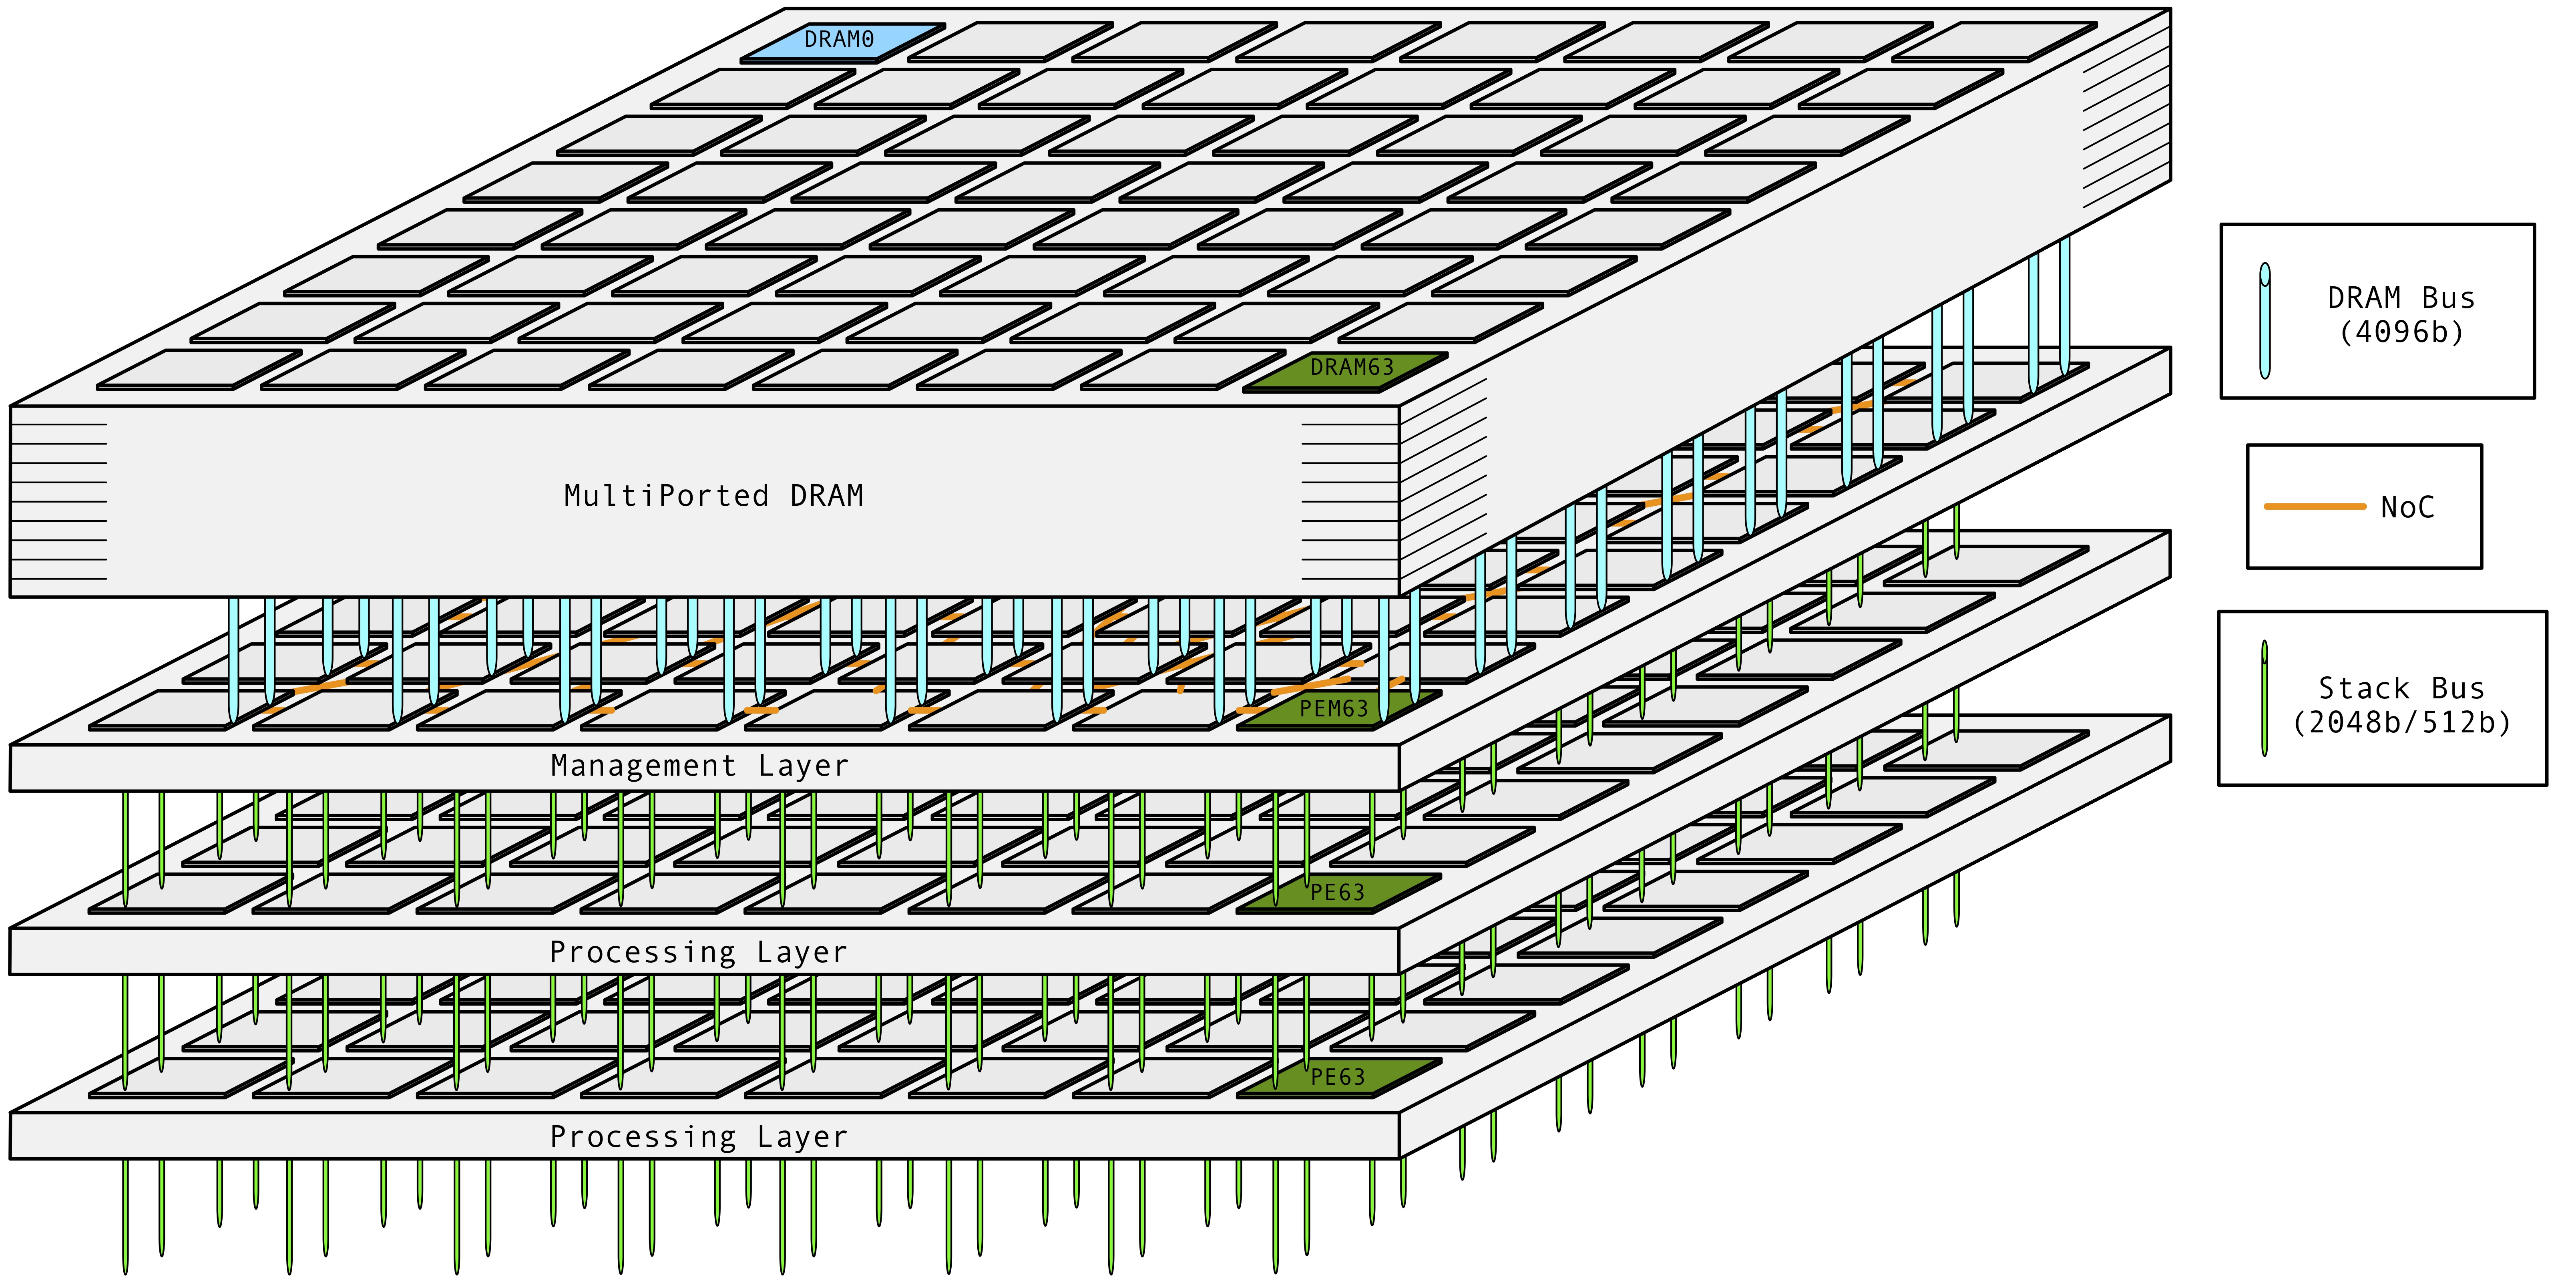
\includegraphics[width=2.75in]{StackDiagram.jpg}}
}
\caption{3DIC System Stack}
\label{fig:3DICStack}
\end{figure}

3D-DRAM has recently become available in standards such as High Bandwidth Memory (HBM) and Hybrid Memory Cube (HMC) and proprietary devices such as the DiRAM4 available from Tezzaron. 
These technologies provide high capacity within a small footprint.

In the case of HBM and DiRAM4, the technology can be combined with additional custom layers to provide a system solution.

The question becomes, can a useful system coexist within the same 3D footprint?

This work targeted a baselne system with:
\begin{itemize}
  \itemsep0em 
  \item target single precision floating point for computations
  \item use the Tezzaron DiRAM4 DRAM for area estimates and memory controller design
\end{itemize}
The work includes customizing the interface to a 3D-DRAM, researching data structures to describe storage of ANN parameters, designing a memory manager with micro-coded instructions and a processing engine (PE) layer.  
The system is designed such that a sub-system, known as a sub-system column (SSC) operates on one of these disjoint memories within the 3D-DRAM  (see figure \ref{fig:diram4Layout}).

When the sub-system columns need to share data or neuron activations, the data is passed between SSCs using a network-on-chip (NoC).

An overview of the various blocks and interconnects are given below:

% ----------------------------------------------------------------------------------------------------
\subsubsection{3D-DRAM}
The targetted 3D-DRAM, the Tezzaron DiRAM4 is a 3D-DRAM employs multiple memory array layers in conjunction with a control and IO layer.
The memory is formed from 64 disjoint sub-memories each providing upwards of 1Gigabit with a total capacity of at least 64 gigabit.
\begin{figure}[!t]
% the [] contains position info e.g. [!t] means here
\captionsetup{width=.9\linewidth}
\centerline{
\mbox{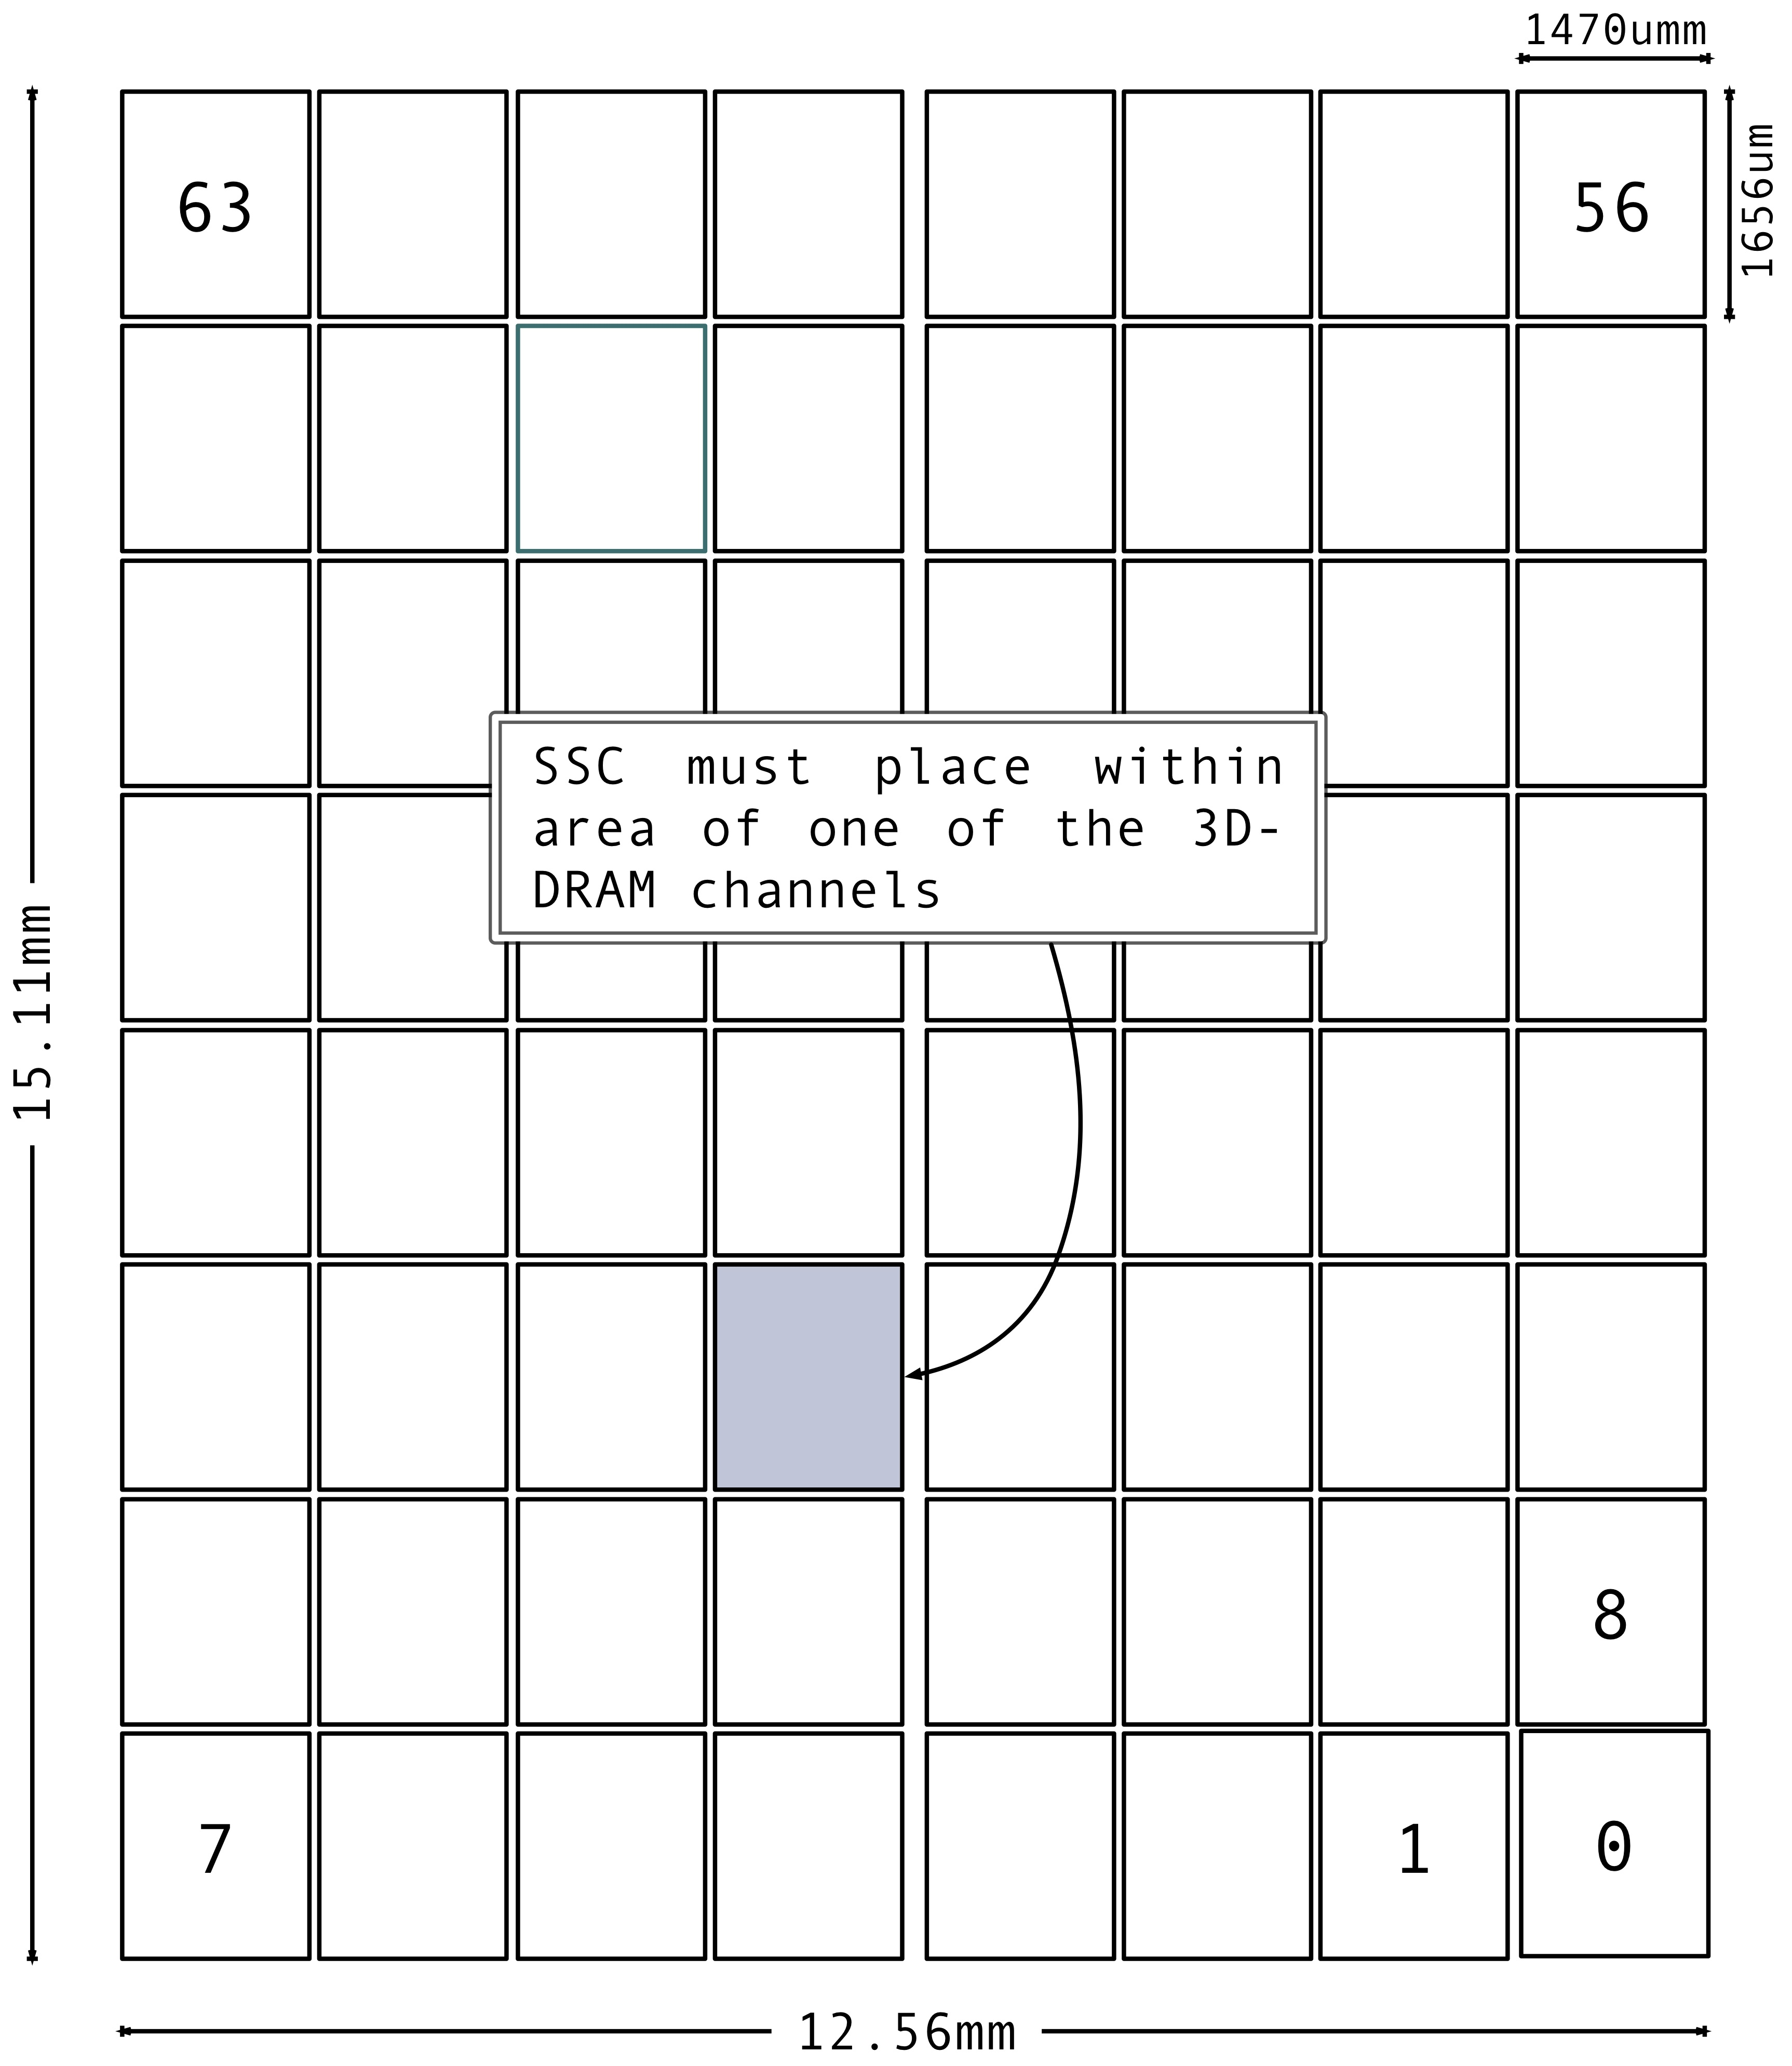
\includegraphics[width=2.5in]{DiRAM4Layout.jpg}}
}
\caption{DRAM Physical Interface Layout showing area for SSC}
\label{fig:diram4Layout}
\end{figure}


% ----------------------------------------------------------------------------------------------------
\subsubsection{Manager Layer}
The Manager block is the main controller in the system. The operations required to process an ANN are formed from individual instructions which are decoded by the Manager. 
These instructions include descriptors to describe memory read operations, processing engine operations and memory write operations. The manager reads these system instructions from an instruction memory, decodes the instruction and configures the various blocks in the system.
The configuration includes:
\begin{itemize}

      \item initiate operand reads from DRAM
      \item prepare the processing engine (PE) to operate on the operands
      \item prepare the result processing engine to take the resulting neuron activations from the PE and write those results back to the DRAM
      \item replicate the resulting neuron activation's to neighbor managers for processing of other ANN layers

\end{itemize}

% ----------------------------------------------------------------------------------------------------
\subsubsection{Processing Layer}
\label{ssec:Processing Layer}
The PE is able to operate on data streamed directly from the DRAM via the Manager layer. The PE is configured by the manager to perform operations on the operand data streamed from the manager. In the baseline system, the main operation is to perform multiply-accumulates on 32 execution lanes of two operands. These operands typically are the pre-synaptic neuron activation's and the connection weights. The PE also performs the activation function on the result of the MAC to generate the neuron activation value. These 32 activation values are sent back to the Manager layer.

% ----------------------------------------------------------------------------------------------------
\subsubsection{Layer Interconnect}
\label{ssec:Layer Interconnect}

The layers are connected using through-silicon-vias (TSVs) which provide high connection density, high bandwidth and low energy.
By ensuring the system stays within the 3D footprint ensures we can take advantage of the huge benefits provided by TSVs.

% ----------------------------------------------------------------------------------------------------
\subsubsection{Inter-Manager Communication}
\label{ssec:Inter-Manager Communication}

During configuration and/or computations, data must be transported between managers. This inter-manager communication is provided by an NoC.
When computing an ANN across multiple processing sub-systems, often neuron activation data must be shared between these SSCs. The SSC includes the DRAM port, the manager and the PE. An NoC within each management block communicates with each adjacent manager using a mesh network. This NoC has a forwarding table that can be reconfigured to provide more efficient routing for a given processing step.

A control and data flow diagram of the stack showing the 64 sub-system columns can be seen in figure \ref{fig:FlowDiagram}.
\begin{figure}[!t]
% the [] contains position info e.g. [!t] means here
\centering
\captionsetup{justification=centering}
\centerline{
\mbox{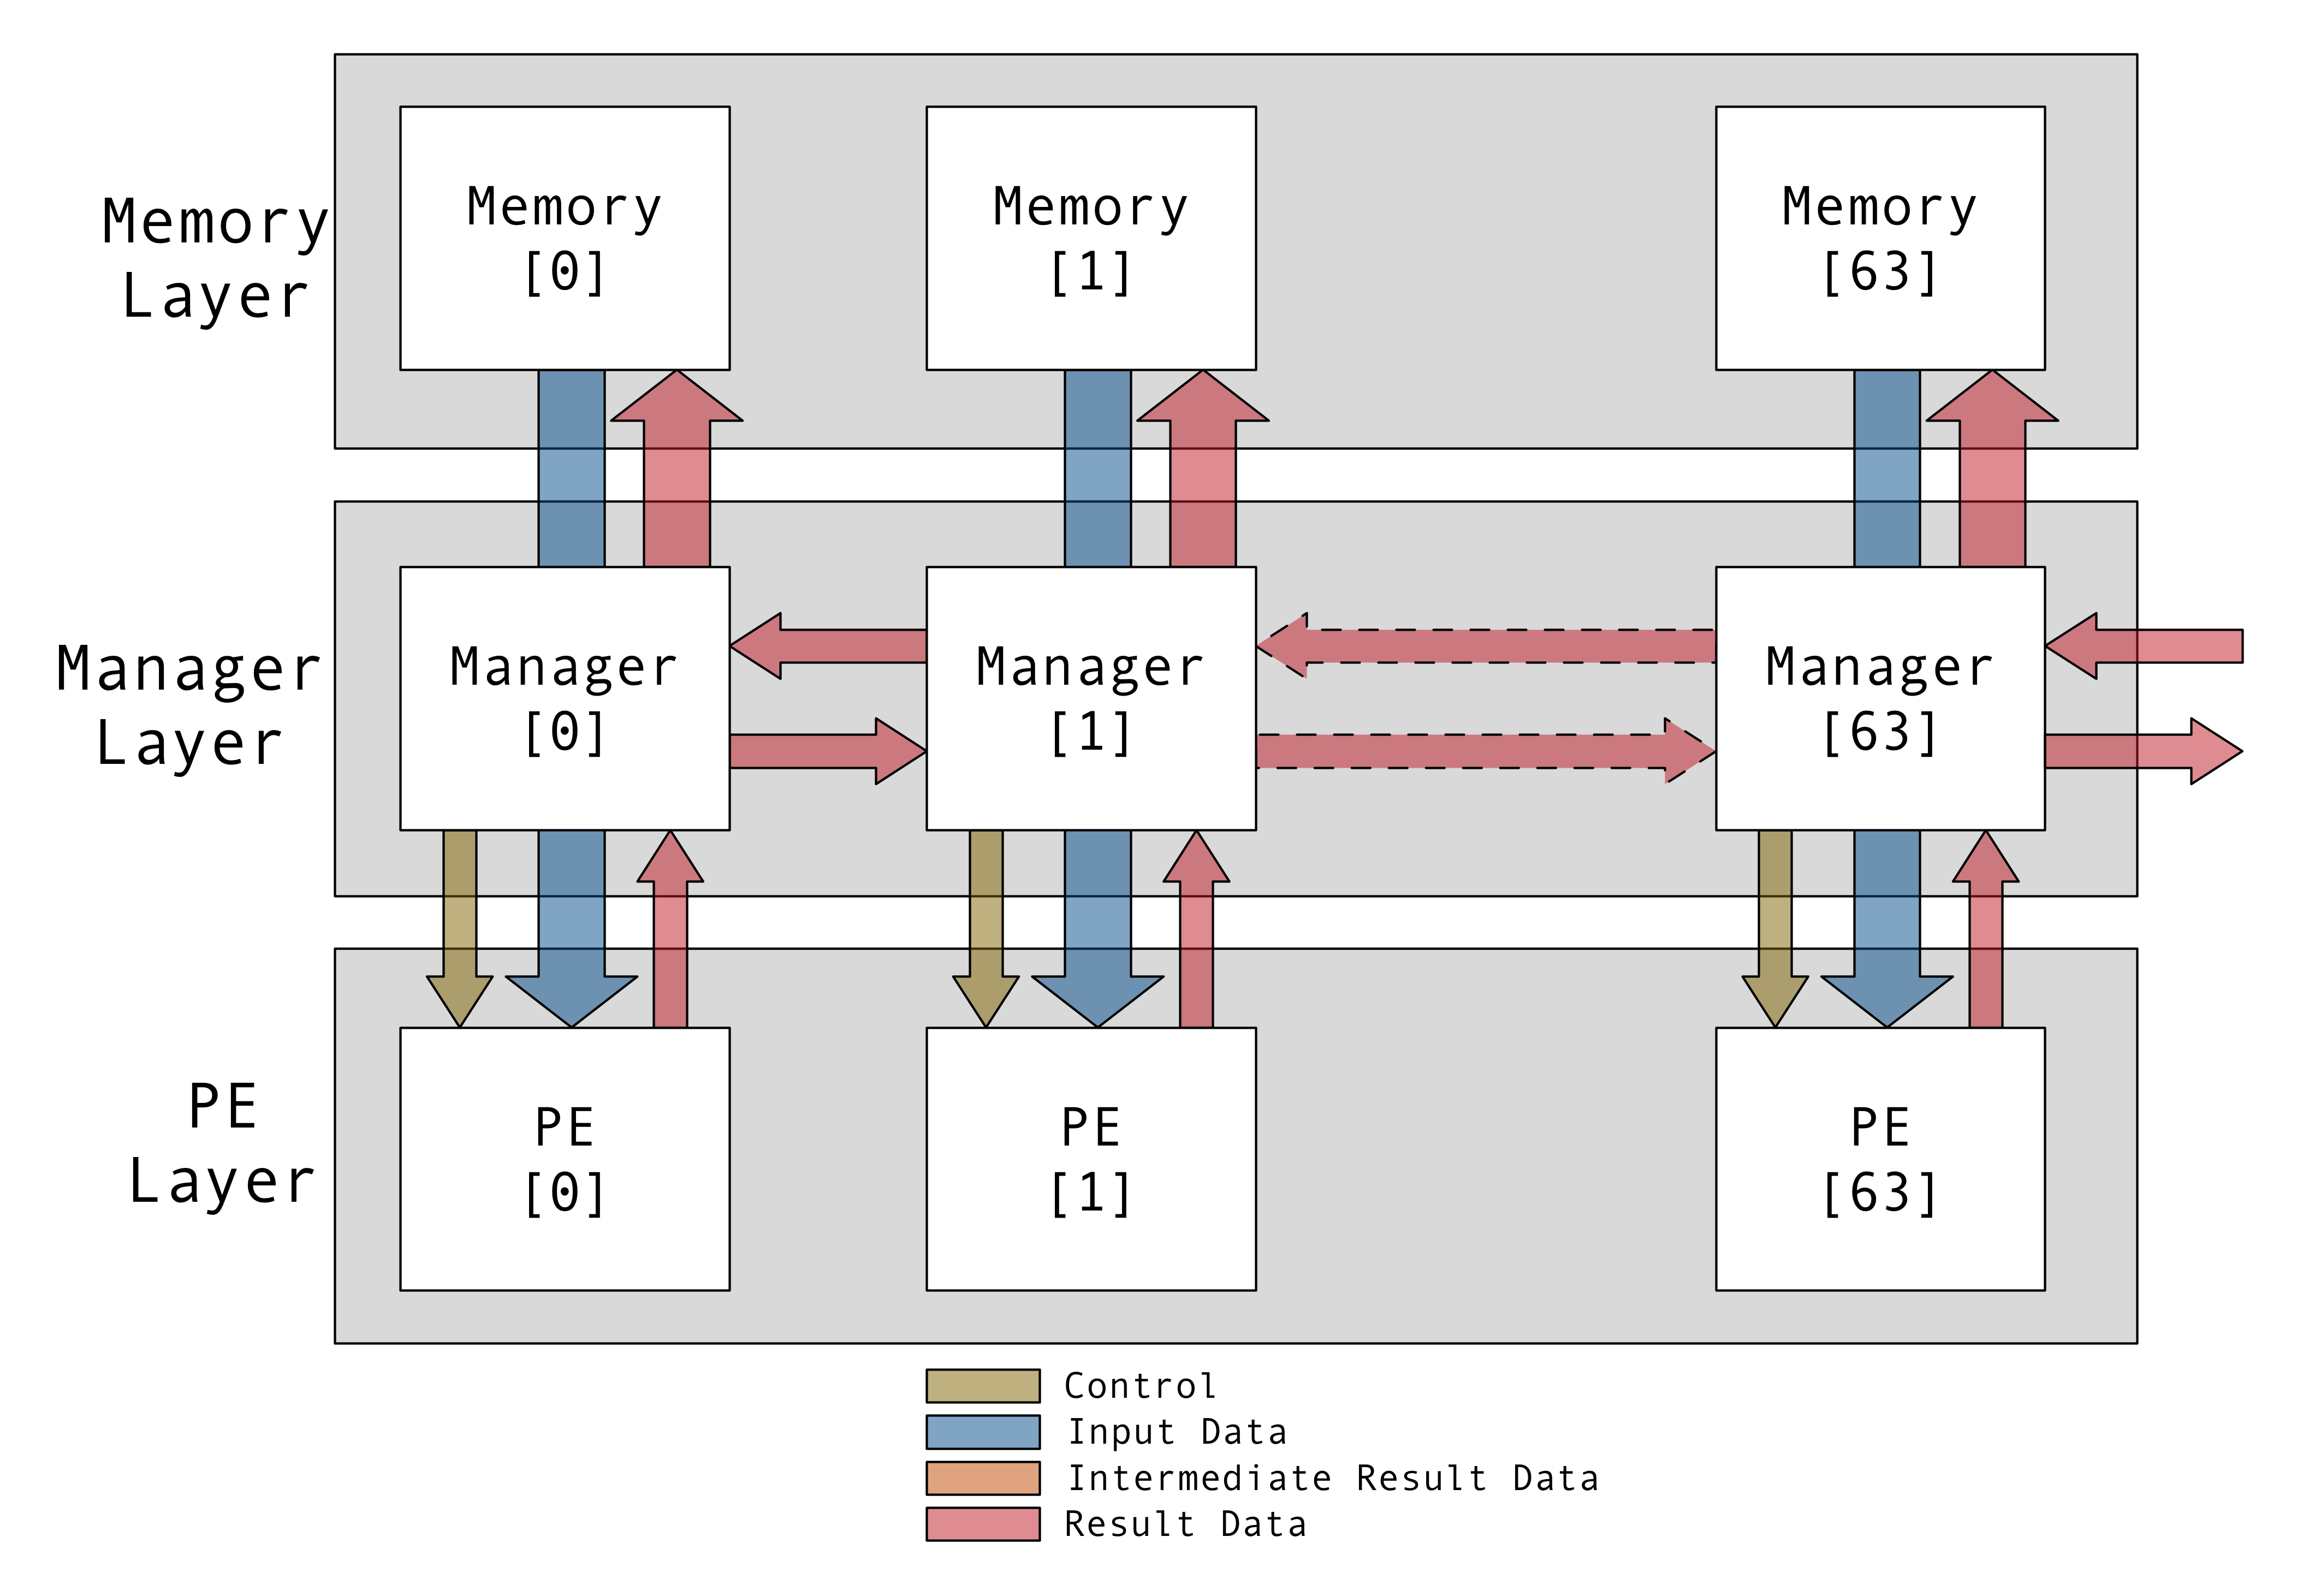
\includegraphics[width=3.0in]{FlowDiagram.jpg}}
}
\center\caption{System Flow Diagram}
\label{fig:FlowDiagram}
\end{figure}


% >>>>>>>>>>>>>>>>>>>>>>>>>>>>>>>>>>>>>>>>>>>>>>>>>>>>>>>>>>>>>>>>>>>>>>>>>>>>> System Operations <<<<<<<<<>>>>>>>>>>>>>>>>>>>>>>>>>>>>>>>>>>>>>>>>>>>>>>>>>><<<<<<<<<<<<<
\section{System Operations}
\label{sec:System Operations}
In the context of this system and AN state calculation, the basic operations to determine the state of a neuron is to:

\begin{itemize}
    \item Inform the Manager and PE which operations are to be performed
    \item Tell the manager to access the states of the pre-synaptic neurons
    \item Tell the manager to access the weights of the connections from the pre-synaptic ANs
    \item Provide the pre-synaptic neuron weights and states to the processing engine execution lanes
    \item Tell the manager where to store the resulting AN state back to memory
\end{itemize}

This work has researched an instruction architecture to describe the above operations which are interpreted by the manager. 

In the baseline system, the manager is not responsible for performing specific algorithm operations but is responsible for coordinating the various data flows and configuration of the modules that make up the system.

The managers primary responsibility is:

\begin{outline}
    \1 Instruction decode
    \1 Internal Configuration messages
    \1 Operand read
    \1 Result write
\end{outline}

In the baseline system, the PE is responsible for the main algorithm operations.

The PE has three major blocks:

\begin{outline}
    \1 Streaming operation function (stOp)
      \2 Processes data from the manager on-the-fly without storing in local SRAM
    \1 SIMD
      \2 processes the data from the stOp function, usually neuron activation such as ReLu
    \1 DMA/local memory controller
      \2 transfer configuration data to PE conroller or to store stOp results to a small local SRAM which can be used for access by SIMD or by the stOp function
\end{outline}
% ----------------------------------------------------------------------------------------------------
% ----------------------------------------------------------------------------------------------------
\subsection{Manager Operations}
\label{sec:Manager Operations}

% ----------------------------------------------------------------------------------------------------
\subsubsection{Instructions}
\label{ssec:Instructions}
The instructions communicate:

\begin{outline}
        \1 To the Manager
            \2 ROI Storage descriptor
            \2 Parameter/Weight Storage Descriptor
                \3 Broadcast or Vectored
            \2 Result write storage descriptor
                \3 include descriptors for all destination managers
        \1 To the PE
            \2 stOp operation
            \2 SIMD operation
            \2 Number of active lanes
            \2 Operand Vector length
\end{outline}

Instructions include information to control the above operations.

Instructions contain sub-instruction called descriptors. These descriptors contain the information to control the various operations associated with the processing of a group of ANs.

The group size is related to the number of execution lanes which for the baseline system is 32. So a group can be anywhere from 1-32. It should be said that unless the group size consistently approaches 32 the system performance will be poor.

An instruction will typically have four descriptors:

\begin{outline}
\renewcommand{\outlinei}{enumerate}
    \1 Operation
    \1 Memory read for operand stream 0
    \1 Memory read for operand stream 1
    \1 Result write
\end{outline}

Note: An operand stream will be reffered to as an argument.

The instruction is actually an n-tuple where the tuple elements are descriptors and the number of elements can vary based on the operation being performed. In figure \ref{fig:instructionTuple} we see the format of a 4-tuple instruction which we use to perform an activation calculation for a group of neurons.

\begin{figure}[!t]
\centerline{
\mbox{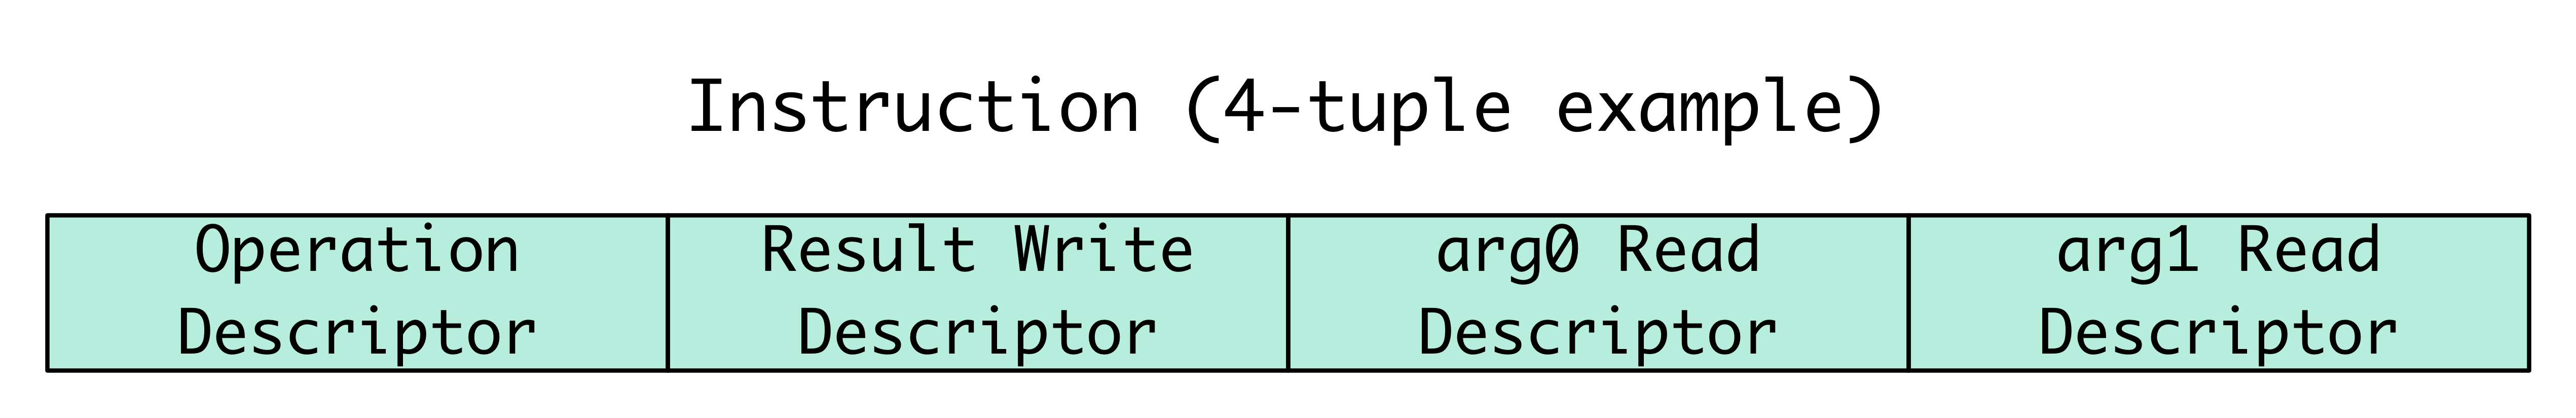
\includegraphics[width=2.75in]{instructionTuple.jpg}}
}
\caption{Instruction 4-tuple}
\label{fig:instructionTuple}
\end{figure}

Now within a descriptor, we need to describe the various options such as storage descriptor pointer, number of operands etc..

Again, we employ a n-tuple format where the first tuple element describes the descriptors operation followed by an m-tuple whose elements contain the options required for the operation.

These option elements are a two-tuple with option and associated value.
In figure \ref{fig:descriptorTuple} we see the format of a 6-tuple descriptor.

\begin{figure}[!t]
\centerline{
\mbox{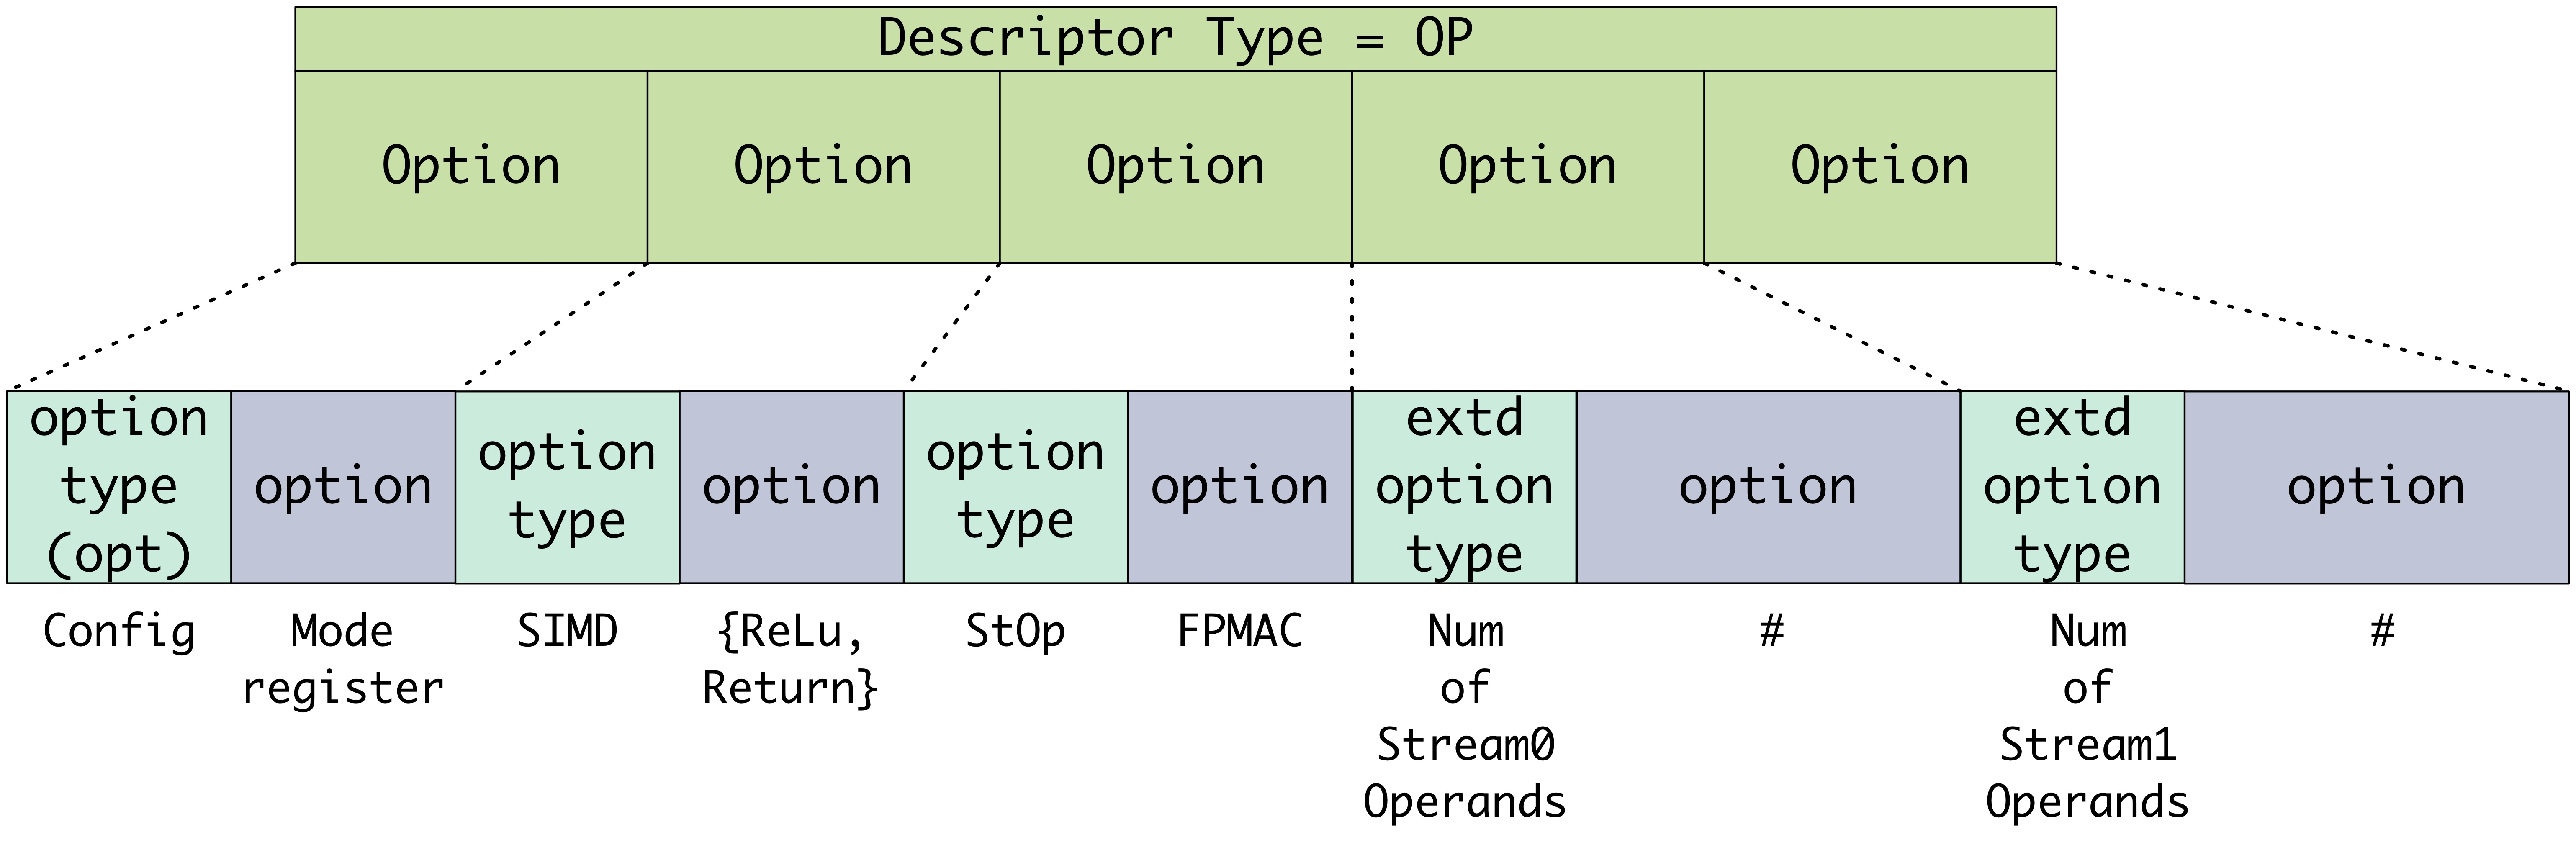
\includegraphics[width=2.75in]{descriptorTuple.jpg}}
}
\caption{Descriptor 6-tuple}
\label{fig:descriptorTuple}
\end{figure}



% ----------------------------------------------------------------------------------------------------
\subsubsection{Accessing of Pre-synaptic AN states and connection weights}
\label{ssec:AccessingANStates}

As was discussed previously, the ANN input and configuration is stored in main DRAM memory. A part of the research is determining how to store the ANN input and parameters in such a way to effectively make use of main DRAM bandwidth. To provide parameters for the up to 32 execution lanes within the PE, we store the AN parameters in consecutive address locations. With one read to the DRAM, we access 128 words. This provides four weights for each of the 32 ANs being processed. These weights are sent to each lane of the PE over four cycles. We will discuss memory efficiency later, but by taking advantage of the multiple DRAM banks along with pre-fetching and buffering, we are able to achieve relatively high efficiency of the available maximum bandwidth.

Although AN parameters (weights) are stored in contiguous memory locations, providing the input state to a particular AN presents us with an interesting problem.

Most often DNNs are represented by layers of ANs whose pre-synaptic neurons are from the previous layer. These previous layers represent the input to a given layer. The first layers input is the actual input to the ANN.


The input can be represented in the form of a 2-D array of AN states. For the sake of generality, the input array elements are considered as AN states.

Any given AN operates on a region of interest (ROI) within the input array.

In figure \ref{fig:roiStorage}, an input to a ANN layer in the form of a 2-D array along with the ROI of two ANs.

\begin{figure}[!t]
\centerline{
\mbox{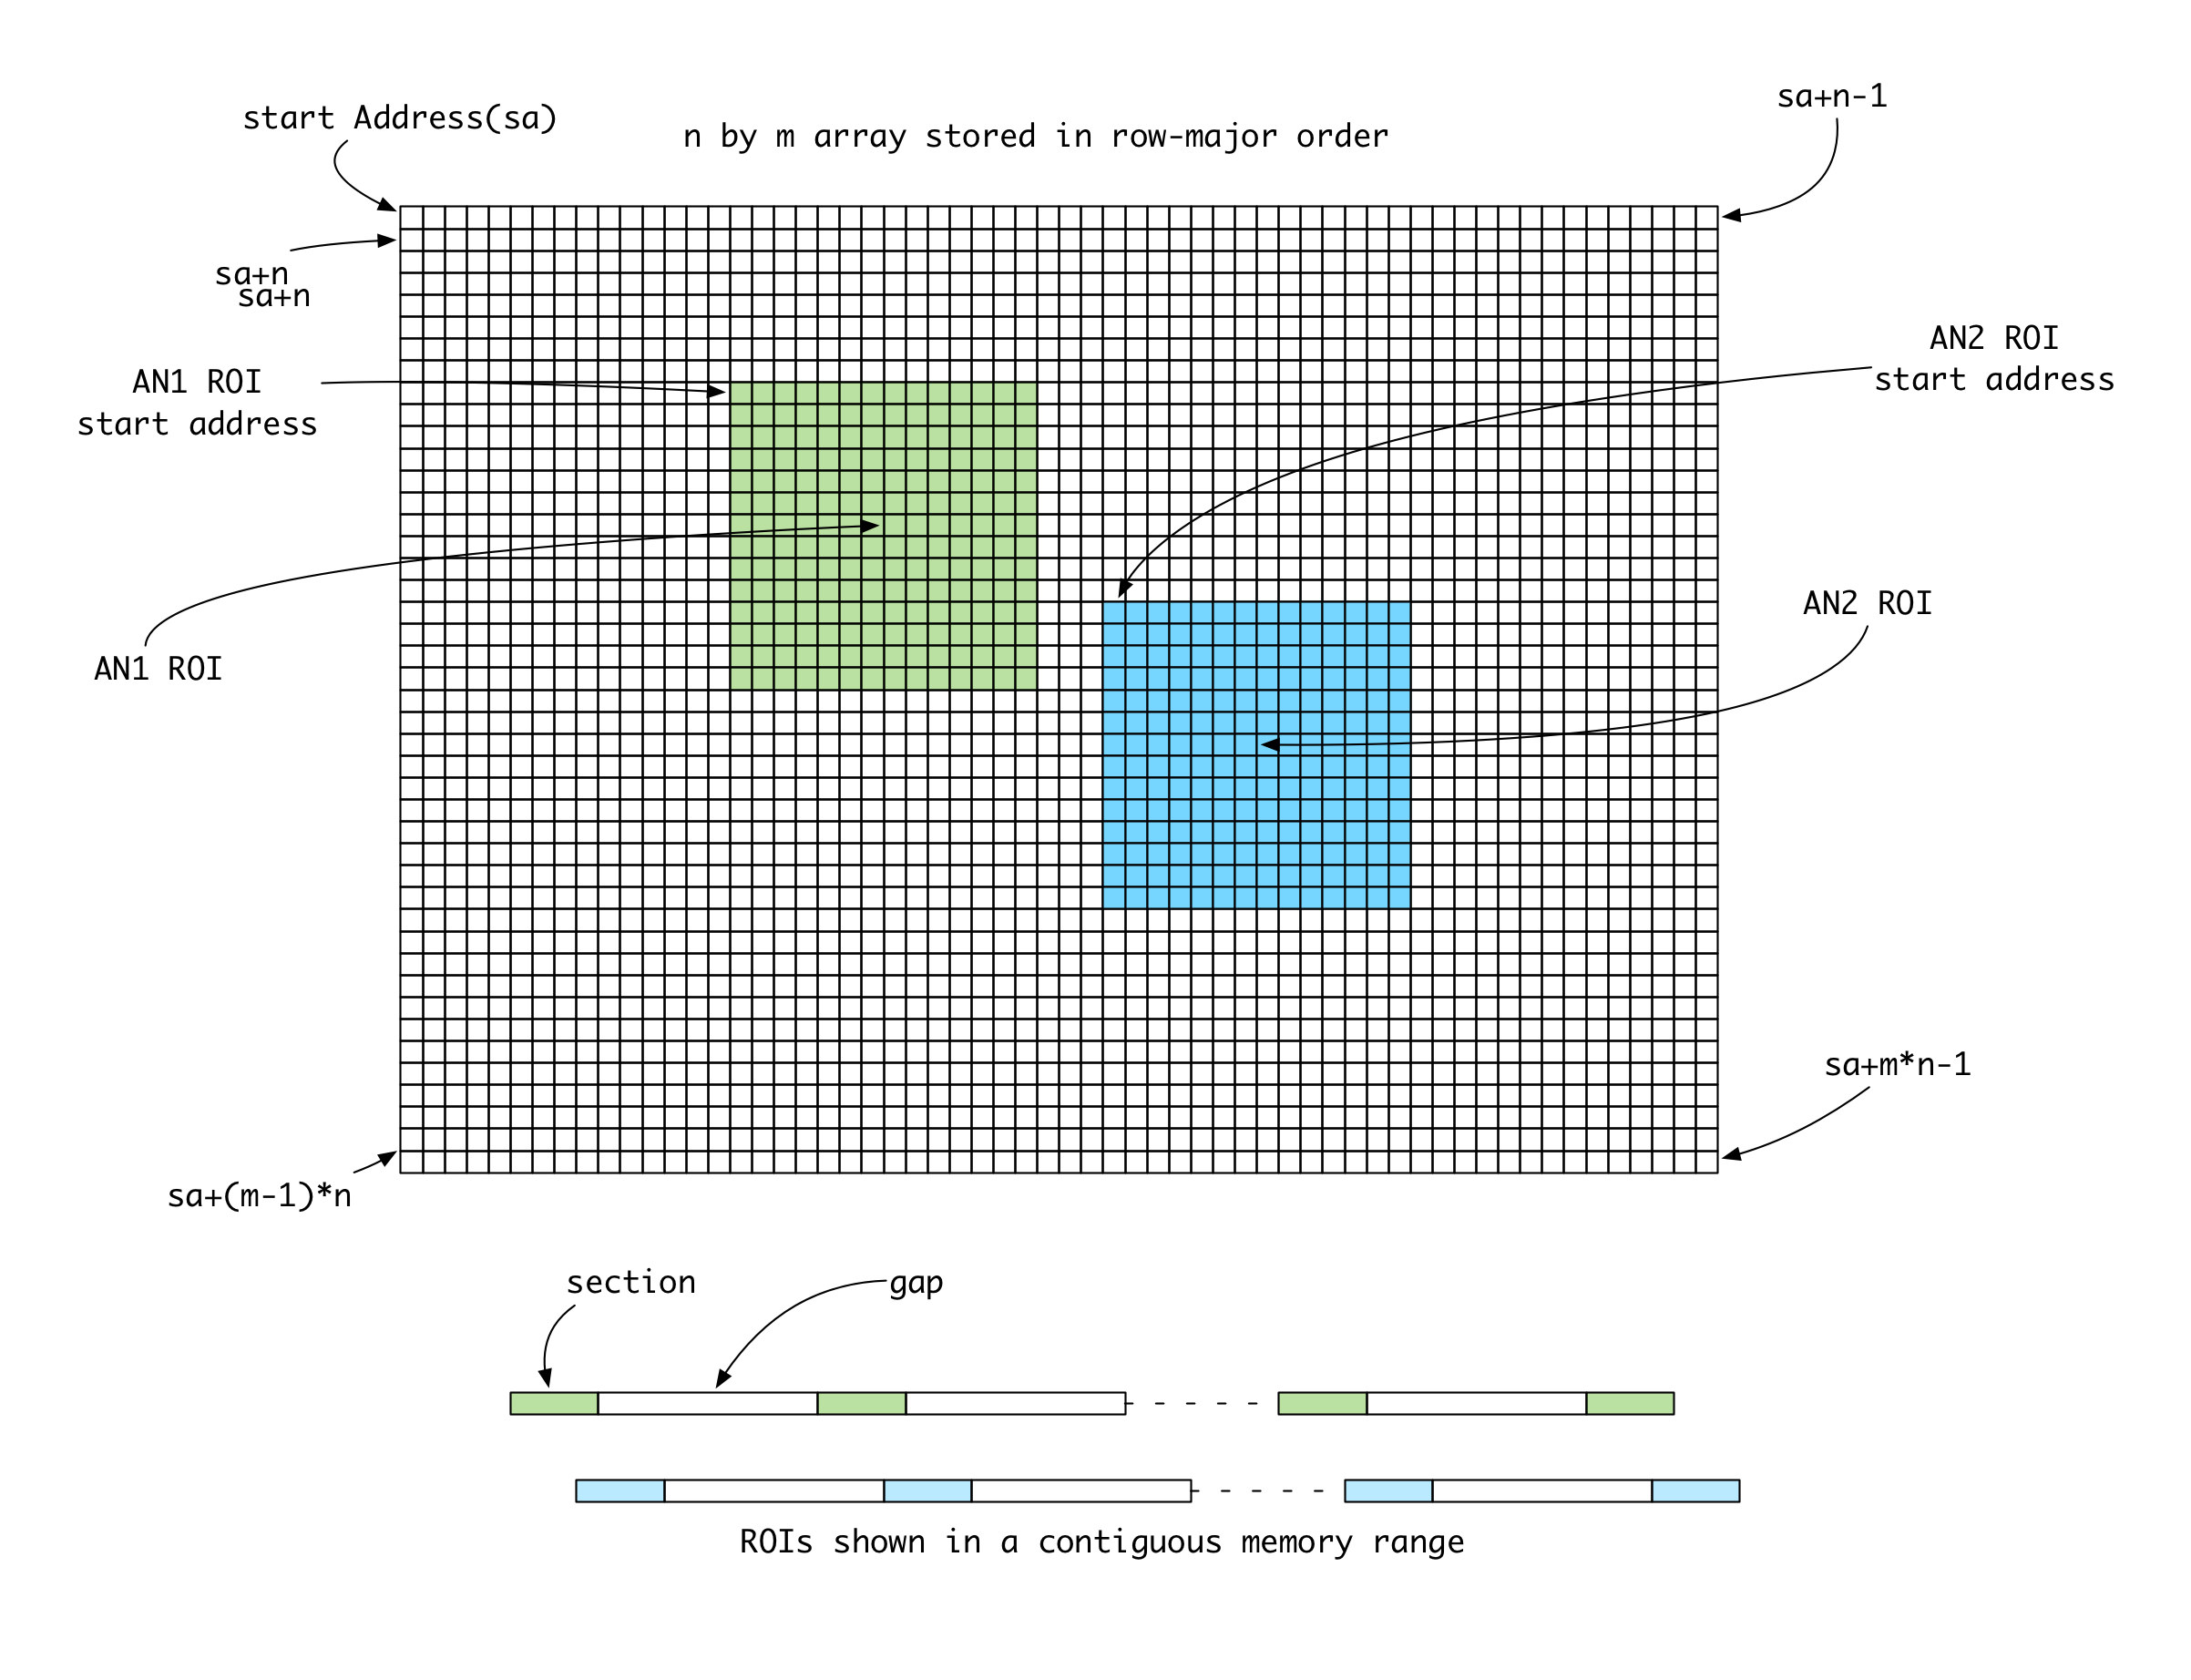
\includegraphics[width=2.75in]{roiStorage.jpg}}
}
\caption{ROI Storage}
\label{fig:roiStorage}
\end{figure}

The various connection weights are stored in multiple contiguous sections. However, its not possible to arrange the input in such a way that each ANs ROI can be stored in contiguous memory locations. The figure above shows a typical ROI arrangement. Assuming the input array is stored in row-major order, an ROI is drawn from disjoint sections of memory. 
These disjoint sections contain a number of AN states and the sections are separated by a gap of a number of memory addresses. When the parameters are accessed when performing a particular operation, the memory controller within the manager must be informed of the start address and the lengths of the sections and gaps. Now this looks problematic, and it is, but in practice groups of ANs share a common ROI. So once we solve the problem of efficiently reading an ROI from the DRAM, that ROI can be shared across a group of ANs

The read efficiency problem is solved by again taking advantage of the DRAMs banks and pages.

This work proposes a data structure to describe these ROI storage locations.

Although disparate groups of ANs may have a different start addresses for their ROI, a commonality is observed in the ROI section lengths and gaps. So for each AN group, the groups ROI starting address is stored along with a pointer to a common set of section length/gaps. This structure is termed a storage descriptor.

This storage descriptor contains, amongst other things the start address of the ROI and a pointer to a section/gap descriptor. Many storage descriptors point to a common section/gap descriptor. This avoids having to have a unique section/gap descriptors for each AN group.

Figure \ref{fig:storageDescriptor} shows the structure of the storage descriptor. The SOD, MOD and EOD are used to delineate each descriptor in memory and stand for start-of-descriptor, middle-of-descriptor and end-of-descriptor.

\begin{figure}[!t]
\centerline{
\mbox{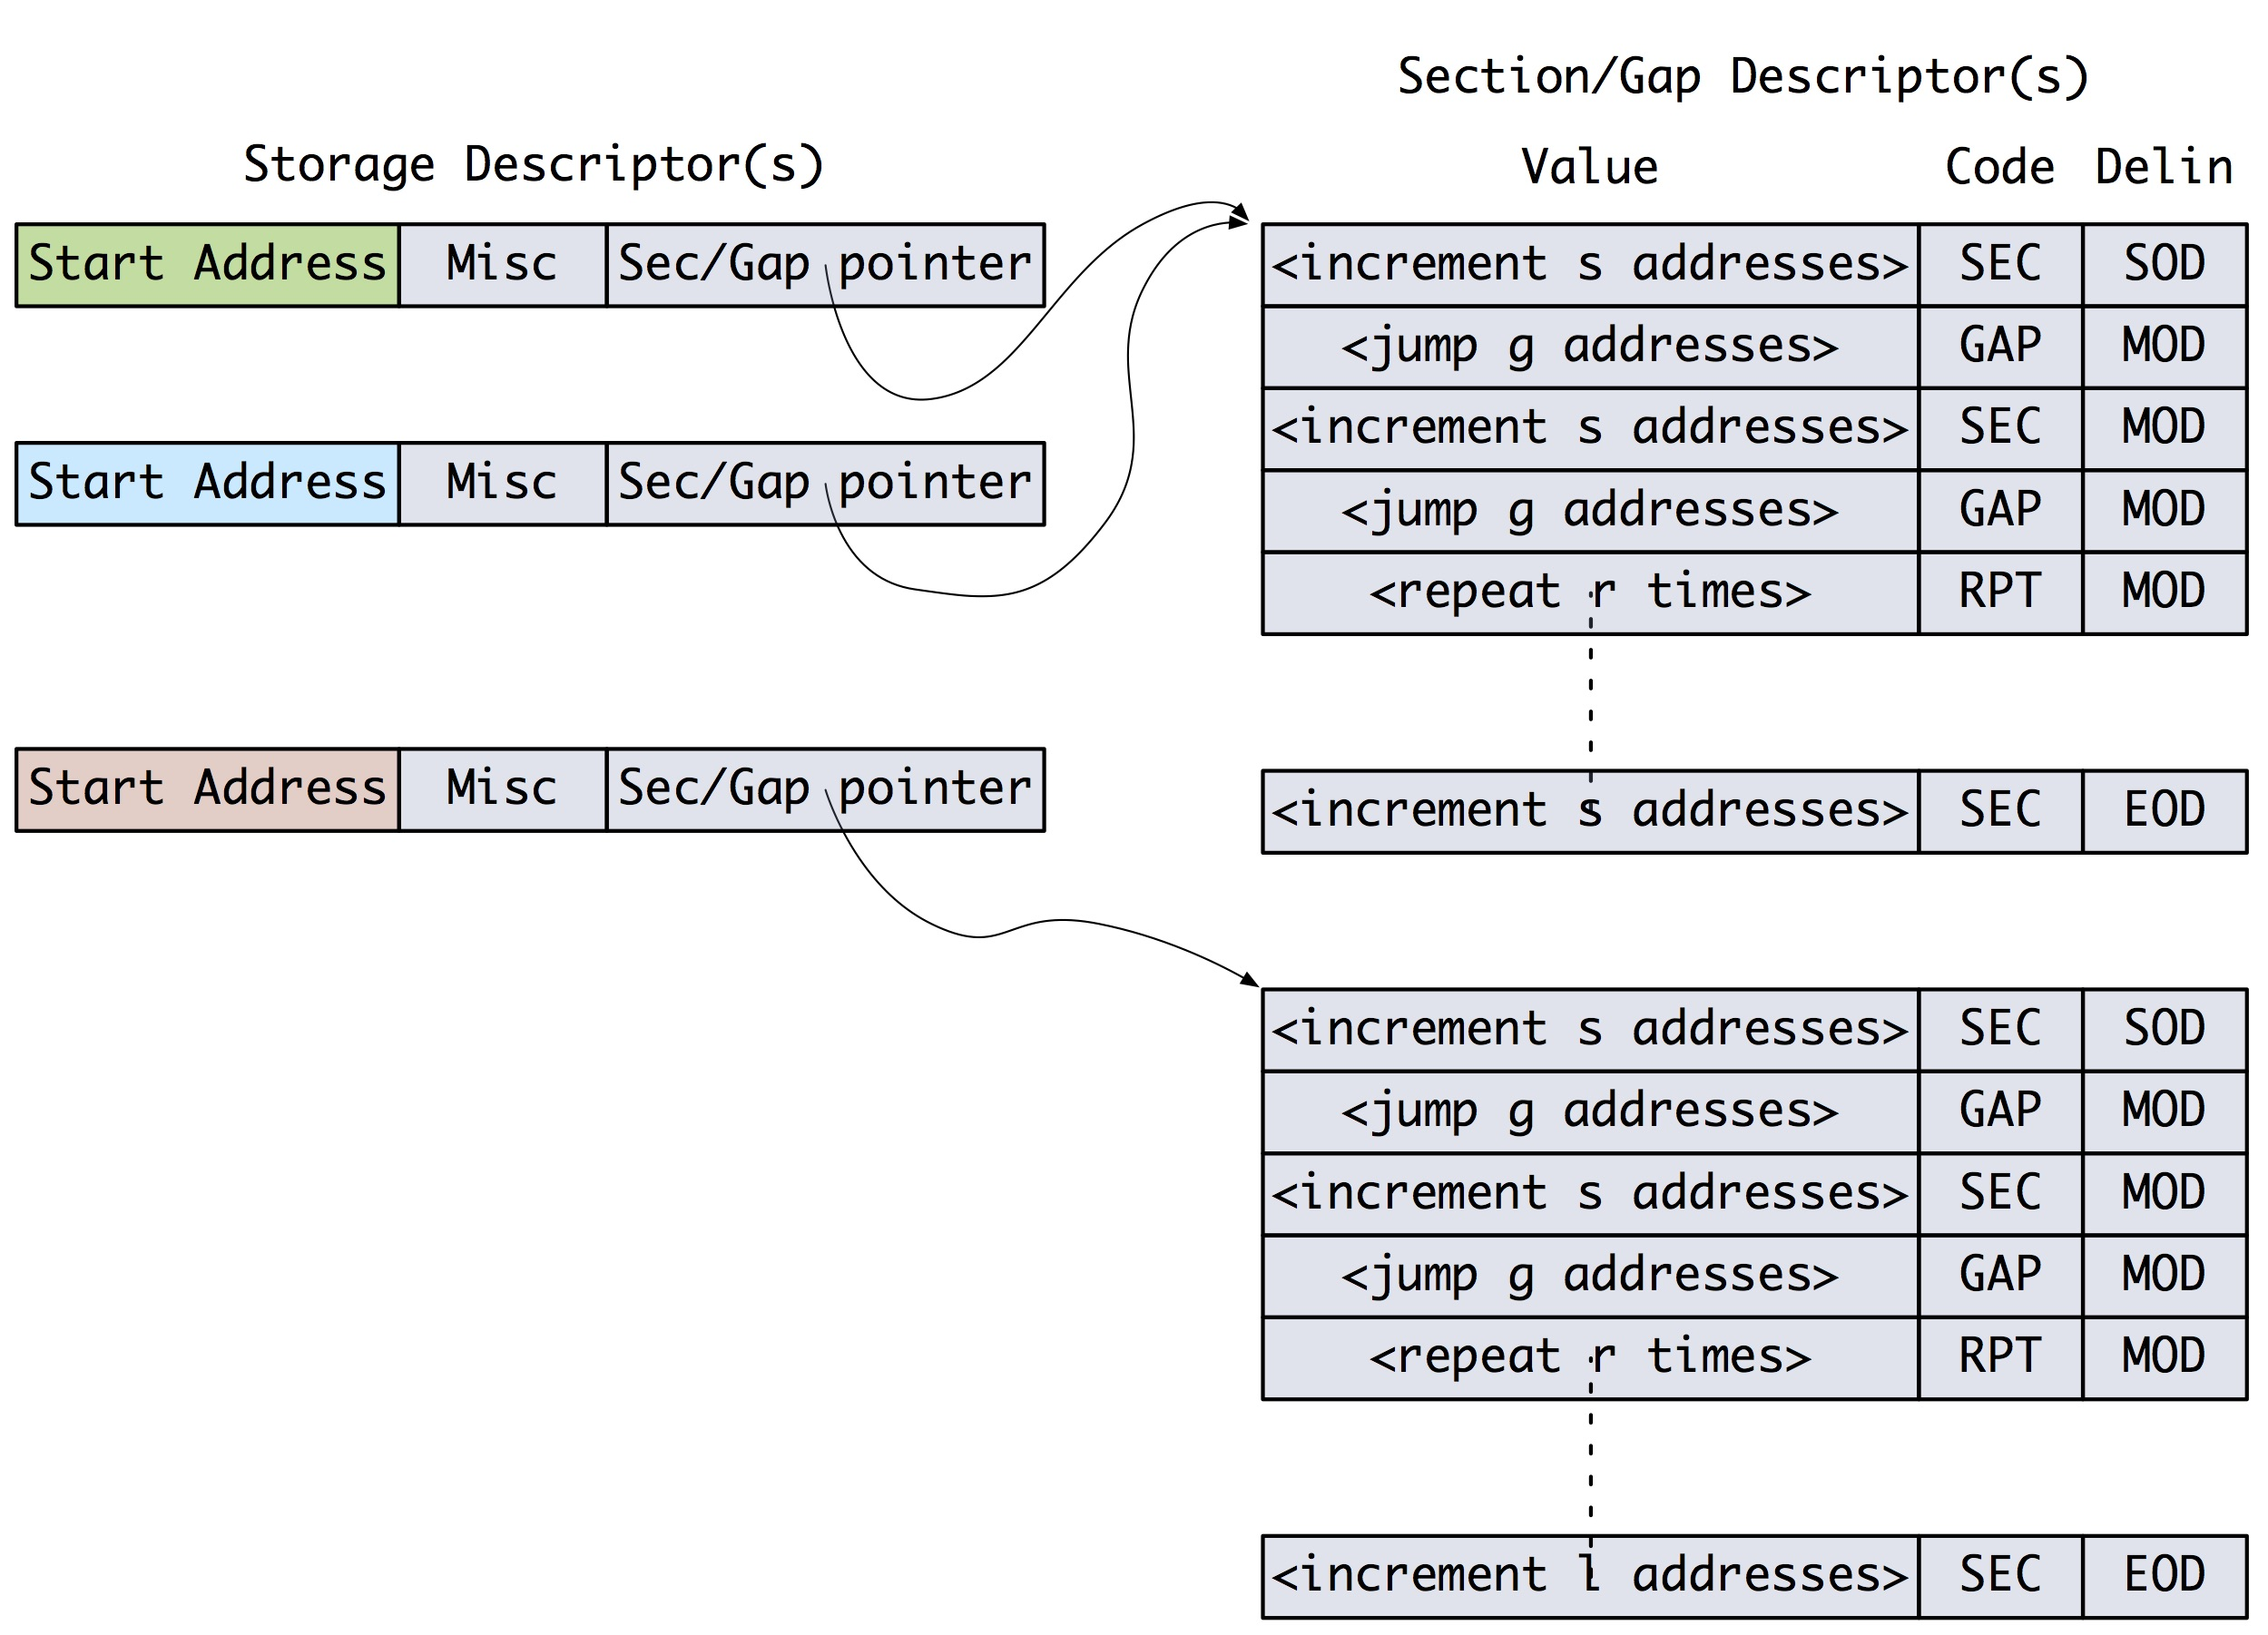
\includegraphics[width=2.75in]{storageDesc.jpg}}
}
\caption{Storage Descriptor}
\label{fig:storageDescriptor}
\end{figure}

% ----------------------------------------------------------------------------------------------------
\subsubsection{Writing AN state results to memory}
\label{ssec:writingANStates}

When the PE has processed the group of ANs, the new AN states are sent back to the manager. The manager will store these back to DRAM most likely in the array format as described earlier.

A significant difference taken advantage of is that for any given operation, the system is writing far less than is being read. For example, the ROI and parameters are usually vectors that will typically exceed 100 elements and in many cases much higher. When an operation is complete, in almost all cases one word per lane is writen back to main memory. 
Now that sounds like writing back has a very small impact on performance but with DRAMs that's not always true.

When the system writes the result of an operation back to memory, it is often writing a small portion of a DRAM page and the nature of the DRAM protocol means this is a very inefficient use of DRAM bandwidth. So although the amount of data written is small the performance impact cannot be ignored.

In addition, in many cases the results from a particular PE has to be provided not only to the PEs local manager but also to other managers. This is handled with a network-on-chip (NoC).

The result storage directives are communicated by using the same storage descriptor mechanism. However, the added complication is because the result will likely have to be replicated to other managers, the storage descriptors must be sent to all destination managers.


% ----------------------------------------------------------------------------------------------------
% ----------------------------------------------------------------------------------------------------
\subsection{PE Operations}
\label{sec:PE Operations}

% ----------------------------------------------------------------------------------------------------
\subsubsection{Streaming Operations (stOp)}
\label{ssec:streamingOps}
The operations performed by the stOp are primarily multiple-accumulate with a transfer to the SIMD or to local memory.

Even though the baseline system focuses on the AN multiply-accumulate followed by a ReLu activation function, the system has built in flexibility into the stOp function to allow other functions to be added

In most cases, the stOp module will operate on the AN state and weights provided by the manager and provide the result to the SIMD.
% ----------------------------------------------------------------------------------------------------
\subsubsection{SIMD}
\label{ssec:SIMD}

The SIMD is a 32-lane processor with some builtin special functions, such as the ReLu operation.

The SIMD will take the result provided by the stOp and perform a ReLu. The result will, in most cases, then transmitted back to the manager.

% ----------------------------------------------------------------------------------------------------
\subsubsection{Configuration}
\label{ssec:peConfiguration}

To configure these operations, two pointers are sent to the PE. These pointers index into a small local memory which provides a program counter (PC) to the function to be performed by the SIMD and a configuration entry for the operation to be performed by the stOp.

The PE is able to perform its operation concurrently on 32-lanes. However, there are cases when less than 32-lanes will be employed. This may occur if the number of ANs being processed is not modulo-32. In this case, the manager provides the number of lanes being processed for any given operation. In addition, the length of the vector of operands is also sent by the manager to the PE.

% >>>>>>>>>>>>>>>>>>>>>>>>>>>>>>>>>>>>>>>>>>>>>>>>>>>>>>>>>>>>>>>>>>>>>>>>>>>>> DRAM Customizable <<<<<<<<<>>>>>>>>>>>>>>>>>>>>>>>>>>>>>>>>>>>>>>>>>>>>>>>>>><<<<<<<<<<<<<
\section{Suggested DRAM Customizations}
\label{sec:Suggested DRAM Customizations}

Accessing a "typical" DRAM involves opening a page in a bank, reading or writing a portion of the contents of the page then closing the page.

Typically a bank may contain of the order of a few thousand pages and a page may contain of the order of a few thousand bits.

Once the page is open, the user accesses a portion of the requested page over a bus. With PCB based DRAMs the bus might vary from four to 16 bits wide, but with 3D DRAMs, such as HBM the bus might be up to 128 bits wide.

Figure \ref{fig:dramBlockDiagram} shows a block diagram of a typical DRAM.

\begin{figure}[!t]
% the [] contains position info e.g. [!t] means here
\centering
\captionsetup{justification=centering}
\centerline{
\mbox{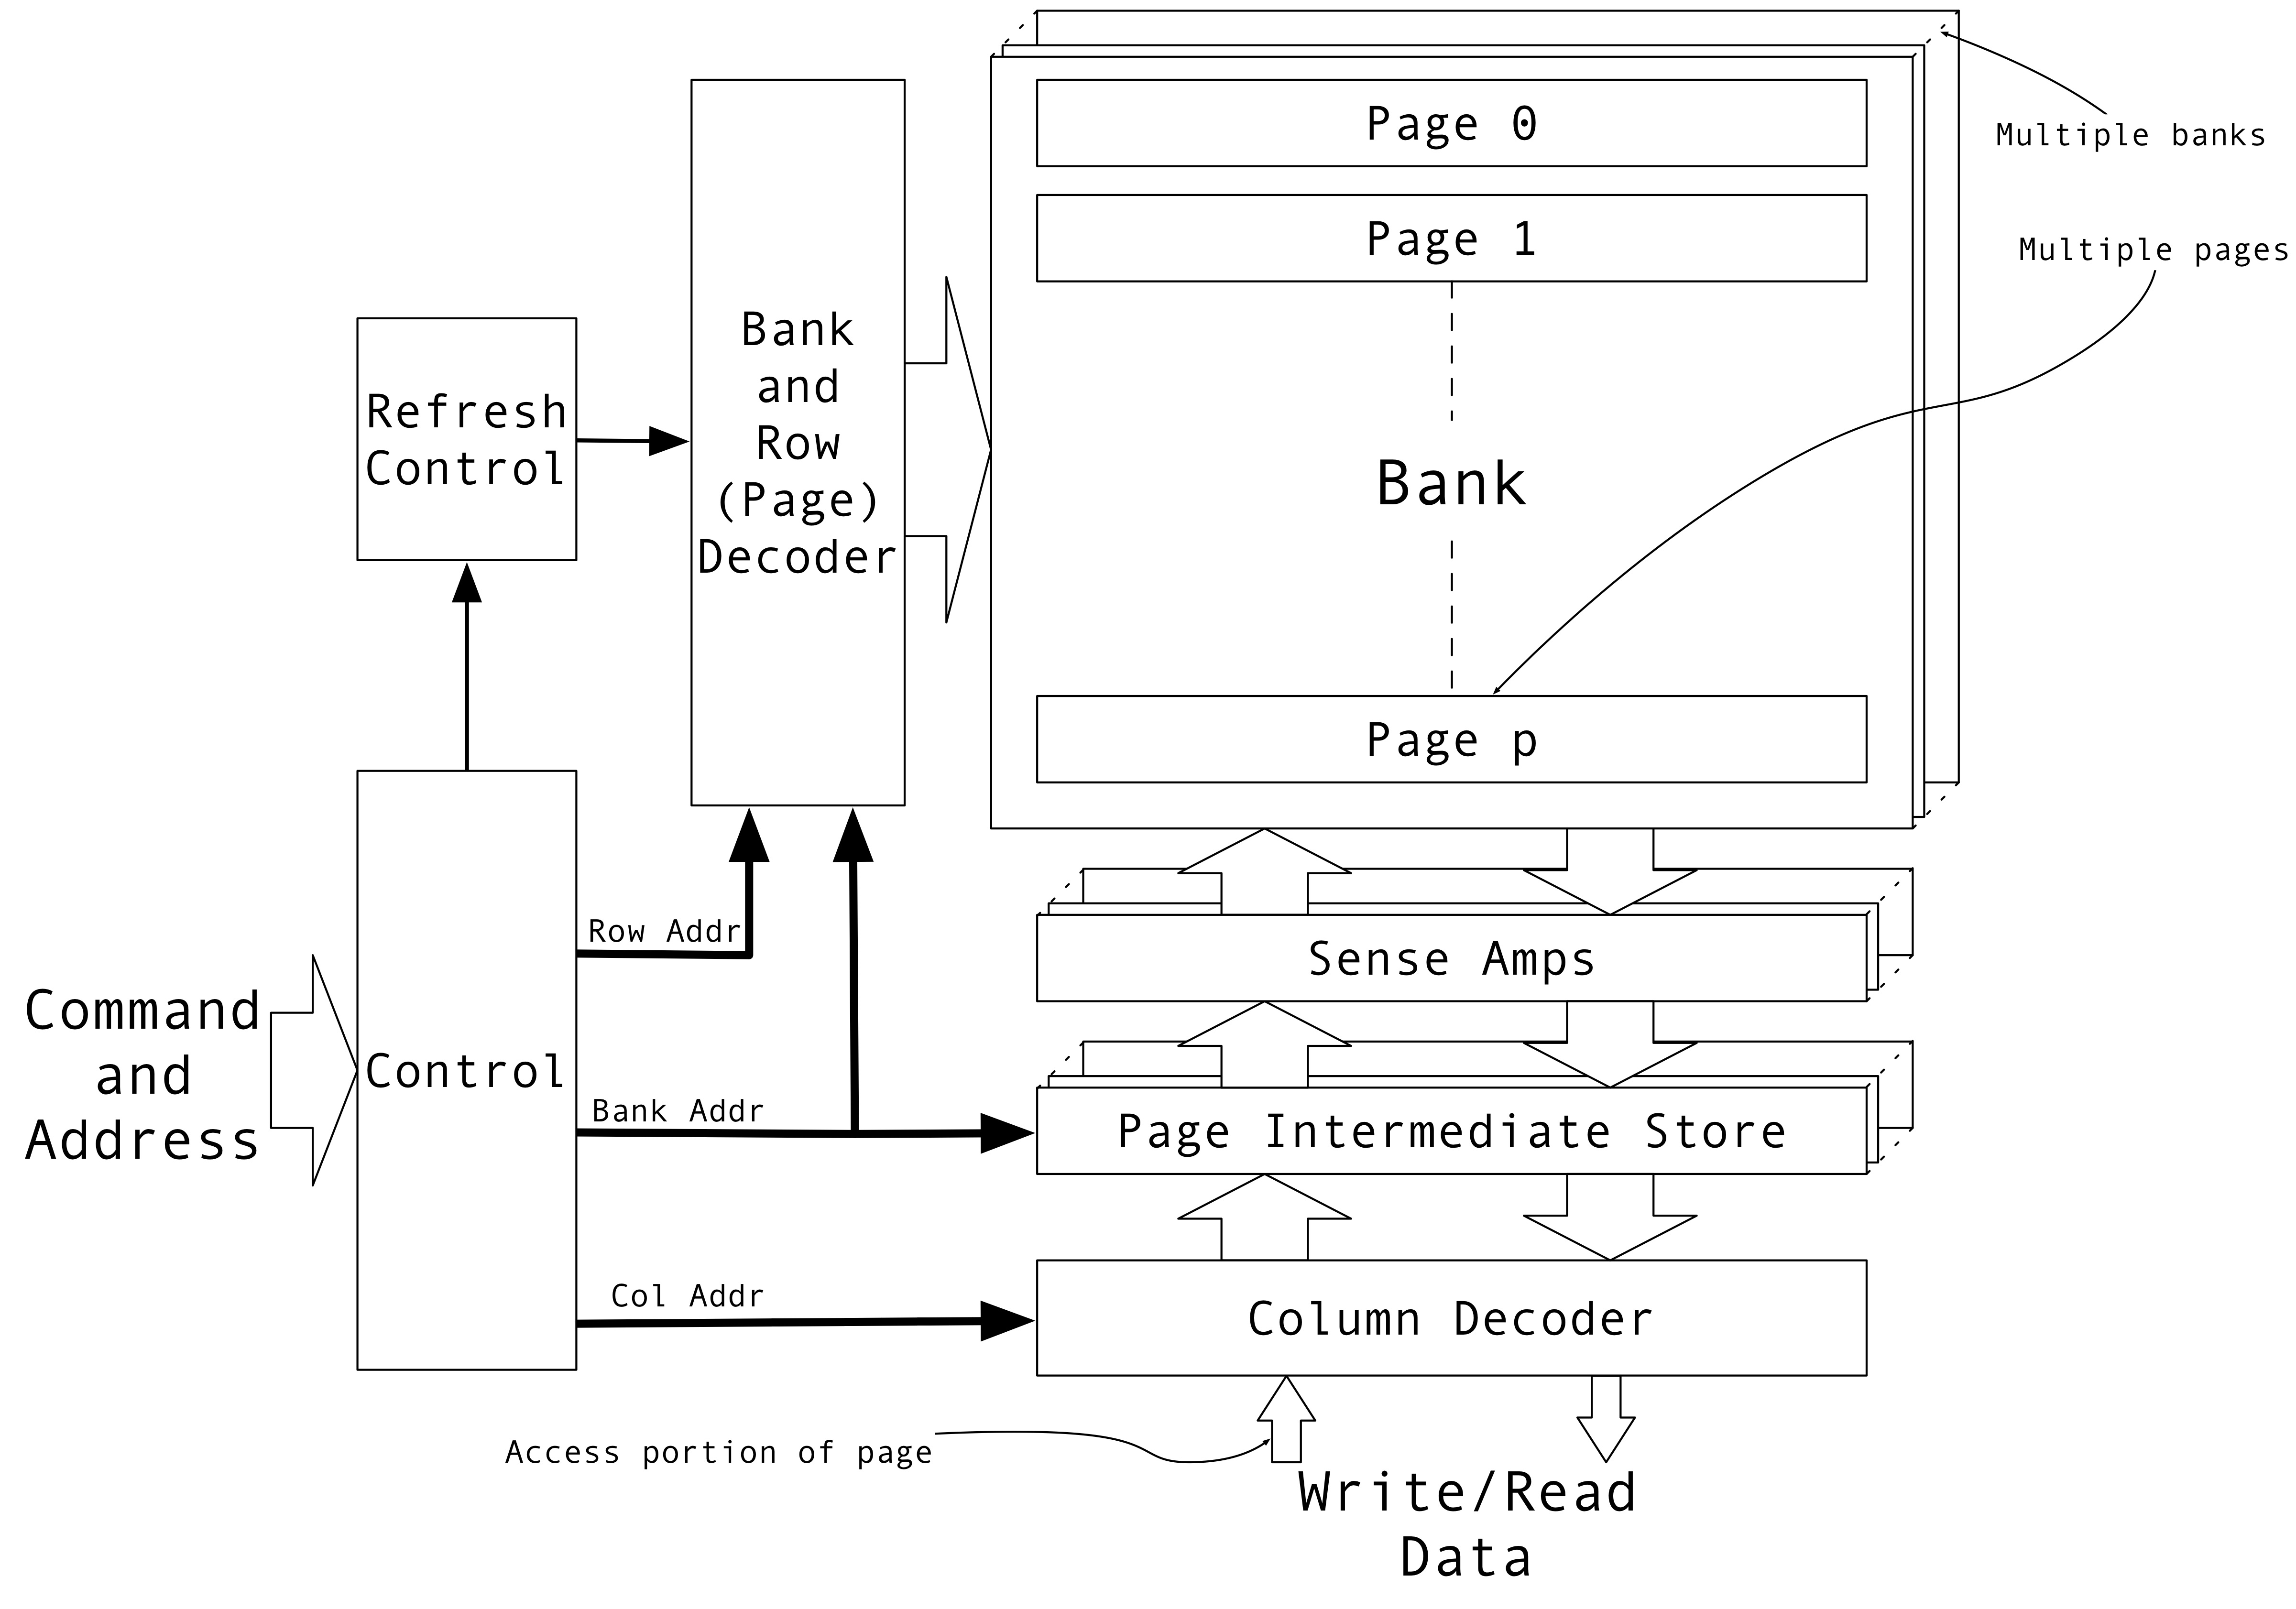
\includegraphics[width=2.75in]{DRAMBlockDiagram.jpg}}
}
\center\caption{Typical DRAM Block Diagram}
\label{fig:dramBlockDiagram}
\end{figure}

\subsection{Expose more of the Page}
\label{sec:exposeMorePage}

This work achieves the increase in bandwidth by proposing that the DRAM expose more of its currently open page.

Without the limitations of having to transfer data beyond the chip stack, this work suggests exposing a larger portion of the page over a very wide bus. By staying within the 3D footprint, this bus can be implemented using fine pitch through-silicon-vias.
(see figure \ref{fig:dramBusChange}).

\begin{figure}[!t]
% the [] contains position info e.g. [!t] means here
\centering
\captionsetup{justification=centering}
\captionsetup{width=.9\linewidth}
\centerline{
\mbox{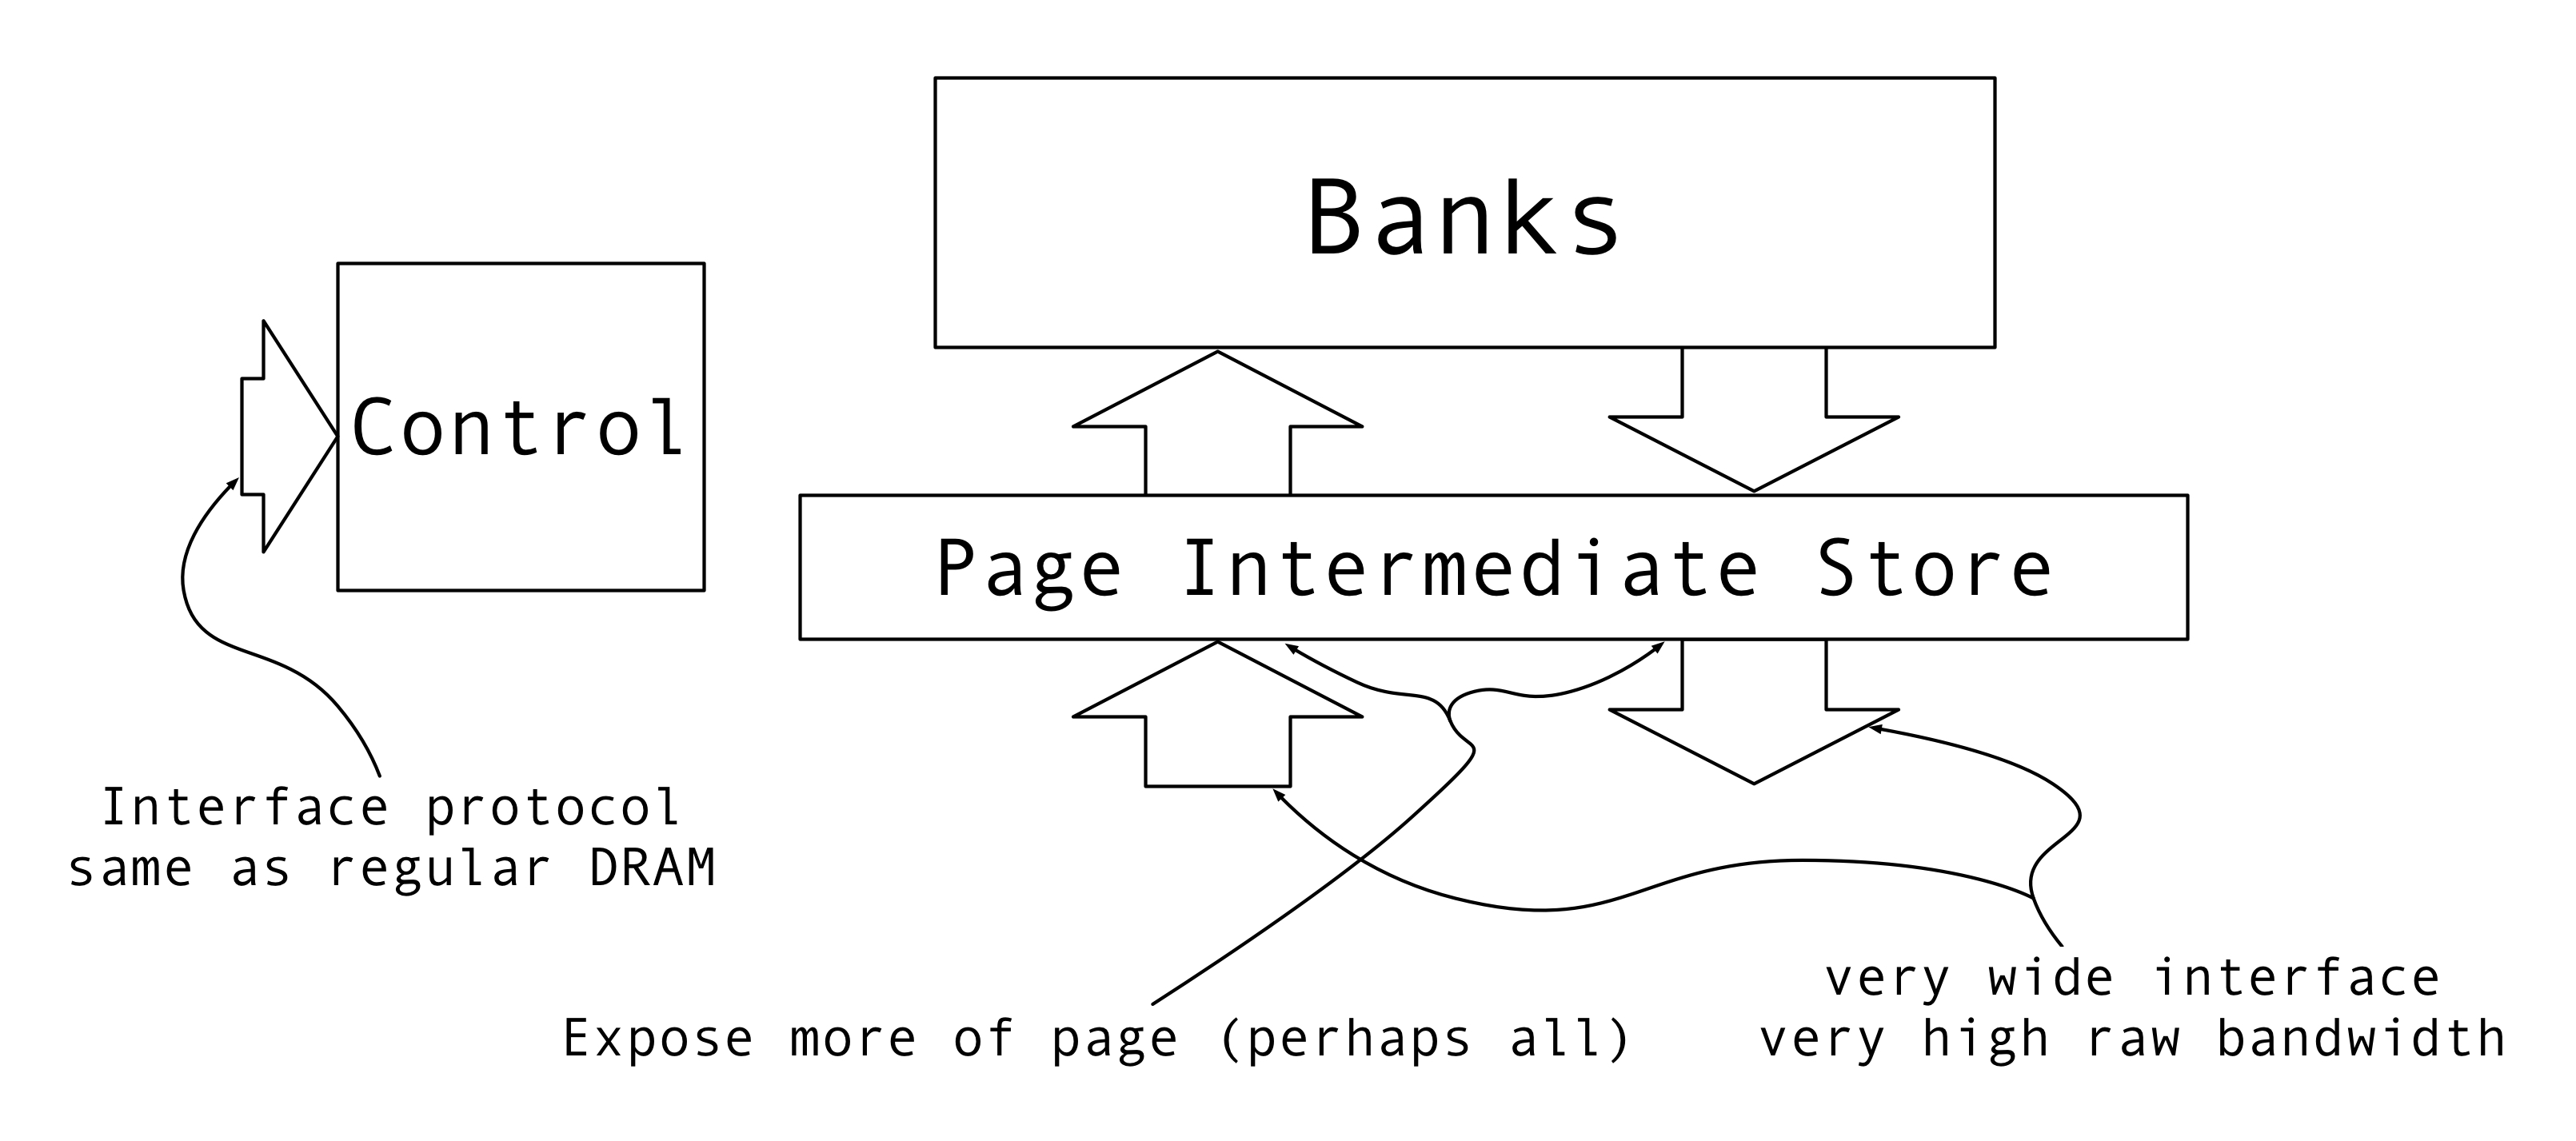
\includegraphics[width=2.75in]{DRAMBusChange.jpg}}
}
\center\caption{Exposing more of the DRAM page}
\label{fig:dramBusChange}
\end{figure}

\subsection{DRAM Write Mask}
\label{sec:dramWriteMask}
When processing an ANN, to compute the activation of an individual AN involves reading the pre-synaptic AN activation's and the weights of the connections between the pre-synaptic ANs and the AN being processed. The activation of the processed AN is written back to memory. The ratio of reads to writes is high, 100's or 1000's to one. Therefore, the system often needs to write a portion of the page back to memory. To avoid a read/modify/write, a customization to the DRAM is the addition of a write data mask to the DRAM write path.


% #######################################################################################################################################
\section{Detailed System Description}
\label{sec:detailedSystemDescription}

A detailed flow diagram and block diagram of the sub-system column can be seen in figures \ref{fig:DetailedFlowDiagram} and \ref{fig:DetailedBlockDiagram} respectively.
\begin{figure}[!t]
% the [] contains position info e.g. [!t] means here
\centering
\captionsetup{justification=centering}
\captionsetup{width=.9\linewidth}
\centerline{
\mbox{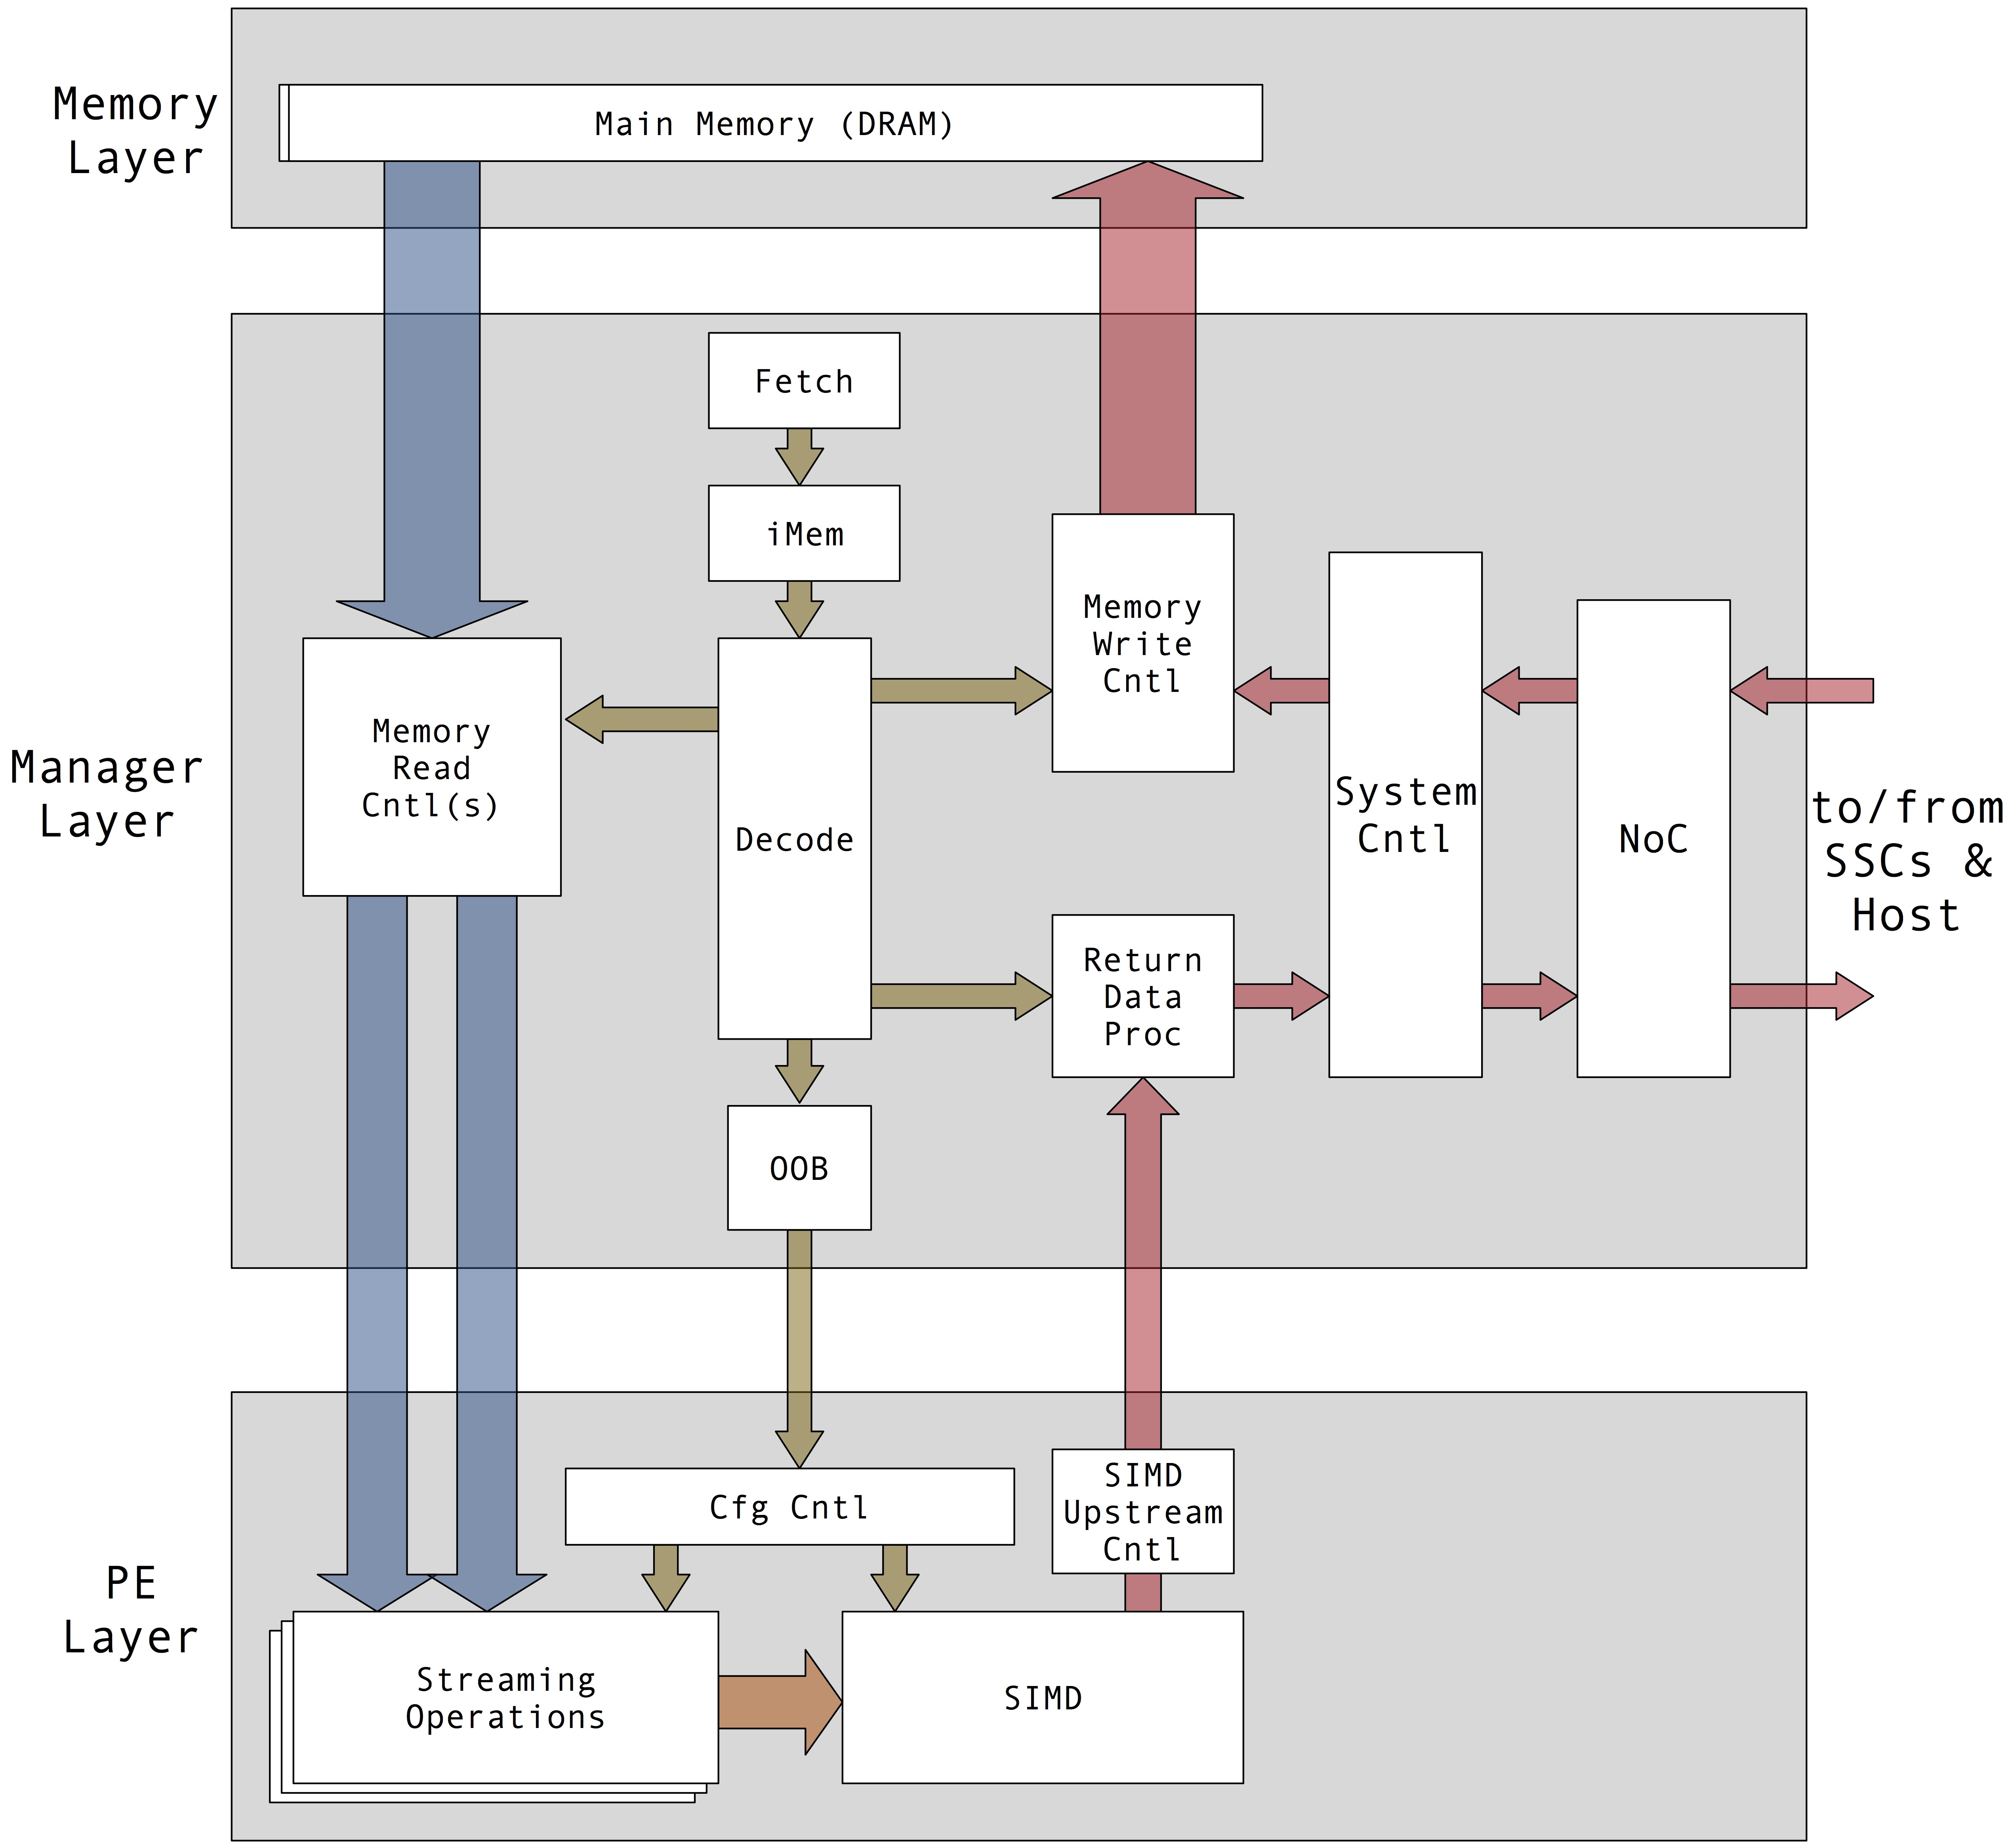
\includegraphics[width=2.75in]{DetailedFlowDiagram.jpg}}
}
\center\caption{Sub-System Column (SSC) Detailed Flow Diagram}
\label{fig:DetailedFlowDiagram}
\end{figure}

\begin{figure*}[!t]
% the [] contains position info e.g. [!t] means here
\centering
\captionsetup{justification=centering}
\centerline{
\mbox{
\includegraphics[width=6.0in]{DetailedBlockDiagram.jpg}}
}
\center\caption{Sub-System Column (SSC) Detailed Block Diagram}
\label{fig:DetailedBlockDiagram}
\end{figure*}

\subsection{Manager}
\label{sec:manager}

\subsubsection{Operation Decode}
\label{ssec:operationDecode}

In figure \ref{fig:DetailedBlockDiagram}, instructions are read from instruction memory and passed to the instruction decoder.

The operation tuple is decoded and a streaming operation (stOp) pointer and a SIMD operation pointer are sent to the PE inside an OOB control packet.

The stOp pointer specifies what streaming operation is to take place on the data directly streamed to the PE. In the baseline system, typically this would be a floating-point multiply accumulate on two arguments, the pre-synaptic neuron states and the pre-synaptic weights.

The SIMD pointer is essentially a program counter that will be invoked when the stOp result is passed to the SIMD.

Note that other types of stOp includes a NOP with a destination of local memory. This allows us to transfer block of instruction or data from the manager to the PE.


\subsubsection{Argument Decode}
\label{ssec:argumentDecode}
The instruction also includes argument descriptors. These descriptors include a storage descriptor pointers that point to a storage descriptor stored in local memory that encodes where data should be read from for the one or two arguments that will be streamed from DRAM to the stOp within the PE. In the case of a AN activation calculation, there are two arguments, the pre-synaptic neuron states and the pre-synaptic weights. The read storage descriptor pointers are passed to the Memory Read Controllers (MRC). The MRCs read the actual storage descriptor from their local memory and immediately start sending read commands to the memory via a Main Memory Controller (MMC). The MMC is not shown in the diagram but essentially takes the memory read requests and converts them into the DRAM read protocol.

As soon as read data is sent back to the MRC via the MMC, that data is aligned with the downstream bus and sent to the 32 Streaming Operations inside the PE.


\subsubsection{Result data Processing}
\label{ssec:resultDataprocessing}
The instruction also includes argument descriptors. These descriptors include a storage descriptor pointers that point to a storage descriptor stored in local memory that encodes where data should be read from for the one or two arguments that will be streamed from DRAM to the stOp within the PE. In the case of a AN activation calculation, there are two arguments, the pre-synaptic neuron states and the pre-synaptic weights. The read storage descriptor pointers are passed to the Memory Read Controllers (MRC). The MRCs read the actual storage descriptor from their local memory and immediately start sending read commands to the memory via a Main Memory Controller (MMC). The MMC is not shown in the diagram but essentially takes the memory read requests and converts them into the DRAM read protocol.

As soon as read data is sent back to the MRC via the MMC, that data is aligned with the downstream bus and sent to the 32 Streaming Operations inside the PE.


\subsubsection{Memory Write Controller}
\label{ssec:memoryWriteController}

The Memory Write Controller (MWC) receives data from to sources, the NoC via the MCNTL and the RDP.

In both cases, the MWC read the actual storage descriptor from their local memory and immediately start forming data that will be written back to main memory.

When the data is formed, a write command is sent to the memory via the MMC. Again, the MMC is not shown in the diagram but takes the memory write requests along with the data and converts them into the DRAM write protocol.

The MWC can only operate on one of the two sources at any one time. However, there are four 4096-bit holding registers where data is formed prior to the write request.

The holding registers have the potential in future to allow aggregation of data from one or more operations to allow a coalesced write back to main memory.


\subsection{Processing Engine}
\label{sec:pe}

\subsubsection{Configuration}
\label{ssec:peConfiguration}

A configuration controller within the PE (PE\_CNTL) takes the OOB packet from the Manager and extracts the stOp and SIMD operation pointers.

The stOp pointer is used to point to a local stOp configuration memory. The memory contains the various configuration data required by the streaming operation controller (stOp\_CNTL). The stOp\_CNTL is not shown.

The stOp\_CNTL configures the:

\begin{outline}
    \1 Operation type
    \1 Number of active execution lanes
    \1 Source of the argument data, which can be downstream data from the manager or from the small local SRAM
    \1 Destination of the result data, which can be the SIMD or the small local SRAM
\end{outline}

The SIMD operation pointer is sent to the SIMD.

\subsubsection{Streaming Operations}
\label{ssec:stOps}

The streaming Operations (stOp) are designed to operate on data passed from the Manager at or near line-rate. If line-rate cannot be maintained, a flow-control mechanism is employed to slow the data from the Manager.

Once the stOp has processed the data, it passes the result to the SIMD. Note in some cases the result can be placed in local SRAM or sent to both SIMD and SRAM.

It should also be stated that while the stOp is processing the current data, the SIMD may be operating on the result of the previous operation. It is expected the SIMD will have completed the previous operation before the stOp completes the current operation, but again, if necessary a flow control mechanism between SIMD and stOP will be engaged if the SIMD is not ready.

\subsubsection{SIMD}
\label{ssec:simd}

The SIMD takes the result data and performs the operation starting at the program counter (PC) indicated by the SIMD operation pointer provided by the PE\_CNTL.

The stOp provides the result to the SIMD via a local register. The result is also written, in most cases to the small local SRAM.

The SIMD performs the specified operation on the data provided by the stOp.

In most cases this will be the AN activation function and in the baseline system is the Rectified Linear function (ReLu).

When the SIMD has completed its operation, it passes the result to the SIMD Upstream controller to be returned to the Manager.

\subsubsection{Result Data}
\label{ssec:result}

The SIMD Upstream Controller (SUI) takes the data and encapsulates it in an Upstream packet. Included in the packet is the tag required by the Return Data processor within the Manager.



% #######################################################################################################################################
% >>>>>>>>>>>>>>>>>>>>>>>>>>> Results <<<<<<<<<<<<<<<<<<<<<<
\section{Results}
\label{sec:Results}
The objectives of this work was to design a system able to accelerate ANNs in customer facing systems implemented at the edge. This means systems that are not designed
to process multiple requests of essentially the same operation.
One assumption is that these systems implement disparate ANNs performing various functions. These assumptions imply that the system is not able to take advantage of local SRAM when processing the ANN.
Another assumption is that the target systems will be space and power constrained.
Finally, this work assumes that implementing multiple disparate ANNs cannot be implemented purely with SRAM and that DRAM is required to store the ANN parameters.

To demonstrate such a system, this work targeted 3DIC technology including 3D-DRAM. This work proposes that if a system can be purely 3DIC, the system can take advantage of the benefits
of 3DIC which inlcudes reduced energy, area and additional bandwidth due to high levels of connectivity.
In addition, this work proposes that if the system is purely 3DIC, then a customized DRAM would provide a significant bandwidth boost over typical implementations using standard DRAM.
This work targeted the Tezzaron DiRAM4 3D-DRAM.

To ensure the system was purely 3DIC, the area of the system Manager and Processing Engine has to stay within the physical footprint of the DRAM.

The target technology node was 28nm. This was chosen because its the technology node employed for some recent GPUs and other ASICs such as \cite{jouppi2017datacenter}.
The design was synthesized using an available 65nm technology node and then scaled to 28nm to demonstrate fitting within the 3DIC footprint.

The primary control and datapaths of the system have been simulated in a system verilog environment. It has been synthesized using a 65nm technology node.
The design has been coded targeting a frequency of $>$\SI{500}{\mega\hertz}. Timing closure and place and route is ongoing. The system has been designed throughout to meet the timing target so minimal changes are expected to meet timing.

As mention previously \eqref{eq:totalBandwidth}, to process multiple useful sized ANNs requires a sustained bandwidth to the PE of the order of ten's of \SI[per-mode=symbol]{}{\tera\bit\per\second}.
%%%%The approximate design targets are shown in Table \ref{tab:DesignTargets}.
%%%%
%%%%\begin{table}[h]
%%%%%  \captionsetup{justification=centering, skip=-5pt}
%%%%  \captionsetup{justification=centering, skip=3pt}
%%%%  \caption{Design targets}
%%%%  \label{tab:DesignTargets}
%%%%  \centering
%%%%%  \begin{center}
%%%%    % [lr] ~ left align col 0 and right align col 1
%%%%    % e.g. 4 columns could be lccr
%%%%    \begin{tabular}{lr}
%%%%      \toprule
%%%%      Parameter         & Target \\
%%%%      \midrule
%%%%      Frequency         & $>$\SI{700}{\MHz}   \\
%%%%      Power             & \SI{\approx 80}{\W}   \\
%%%%      Bandwidth         & \SI[per-mode=symbol]{\approx 64}{\tera\bit\per\second} \\
%%%%      Overall Die Area  & \SI{175}{\mm^2} \\
%%%%      \bottomrule
%%%%    \end{tabular}
%%%%%  \end{center}
%%%%\end{table}

The Manager and PE have been place and routed as shown in figure \ref{fig:Manager and PE Die layouts}. Although the design is yet to close timing, the parasitics
were extracted from these layouts and simulated against a group of operations. The simulation generated an activity file which was then used by the 
Synopsys\textregistered ~Primetime-PX\texttrademark ~power analysis tool to obtain power and bandwidth estimates. Those estimates were used to estimate power dissipation for operating frequencies of \SI{500}{\mega\hertz} and \SI{700}{\mega\hertz}
which are shown in table \ref{tab:Simulation-based estimates}.

\begin{table}[h]
%  \captionsetup{justification=centering, skip=-5pt}
  \captionsetup{justification=centering, skip=3pt}
  \caption{Simulation-based estimates}
  \label{tab:Simulation-based estimates}
  \centering
%  \begin{center}
    % [lr] ~ left align col 0 and right align col 1
    % e.g. 4 columns could be lccr
  \begin{adjustbox}{width=0.45\textwidth}
    \begin{tabular}{cccccc}
          \toprule
                            % \multicolumn{4}{c}{3D-DRAM Simulation-based estimates}   \\
                         &                       &  Usable    &          &          &  \\  %\cline{1-1}
                         &                       &   DRAM     & Expected &          &  \\  %\cline{1-1}
                   Tech  & Freq                  & Bandwidth  &  Power   &  FLOPS   &  \\  %\cline{1-1}
          \hline  % instead of \midrule %midrule doesnt overlap with column lines
                   28    & \SI{500}{\mega\hertz} & \SI[per-mode=symbol]{\sim 46}{\tera\bit\per\second}&53W&  \SI[per-mode=symbol]{2.0}{\tera FLOP\per\second}\\ %\cline{2-2}
                   28    & \SI{700}{\mega\hertz} & \SI[per-mode=symbol]{\sim 64}{\tera\bit\per\second}&73W&  \SI[per-mode=symbol]{2.8}{\tera FLOP\per\second}\\ %\cline{2-2}
          \bottomrule
    \end{tabular}
\end{adjustbox}
%  \end{center}
\end{table}


%%%%\begin{table}[h]
%%%%%  \captionsetup{justification=centering, skip=-5pt}
%%%%  \captionsetup{justification=centering, skip=3pt}
%%%%  \caption{Design targets}
%%%%  \label{tab:DesignTargets}
%%%%  \centering
%%%%%  \begin{center}
%%%%    % [lr] ~ left align col 0 and right align col 1
%%%%    % e.g. 4 columns could be lccr
%%%%    \begin{tabular}{lccccc}
%%%%          \toprule
%%%%                            %& \multicolumn{4}{c}{Technology}   \\
%%%%                            &       &       &  Usable    &          &  \\  %\cline{1-1}
%%%%                            &       &       &   DRAM     & Expected &  \\  %\cline{1-1}
%%%%                            & Tech  & Freq  & Bandwidth  &  Power   &  \\  %\cline{1-1}
%%%%          \hline  % instead of \midrule %midrule doesnt overlap with column lines
%%%%                  3D-System & 28    & \SI{700}{\mega\hertz}      &       \SI[per-mode=symbol]{\sim 64}{\tera\bit\per\second}   &  73W   &  \\ %\cline{2-2}
%%%%                  NVidia    & 28    &       &  $\ll$\SI[per-mode=symbol]{1.28}{\tera\bit\per\second} &  100W  &  \\
%%%%                  TPU       & 28    &       &  $<$  \SI[per-mode=symbol]{224}{\giga\bit\per\second}  &  40W   &  \\
%%%%          \bottomrule
%%%%    \end{tabular}
%%%%%  \end{center}
%%%%\end{table}



\begin{figure}
\centering
\begin{subfigure}{.25\textwidth}
  \centering
  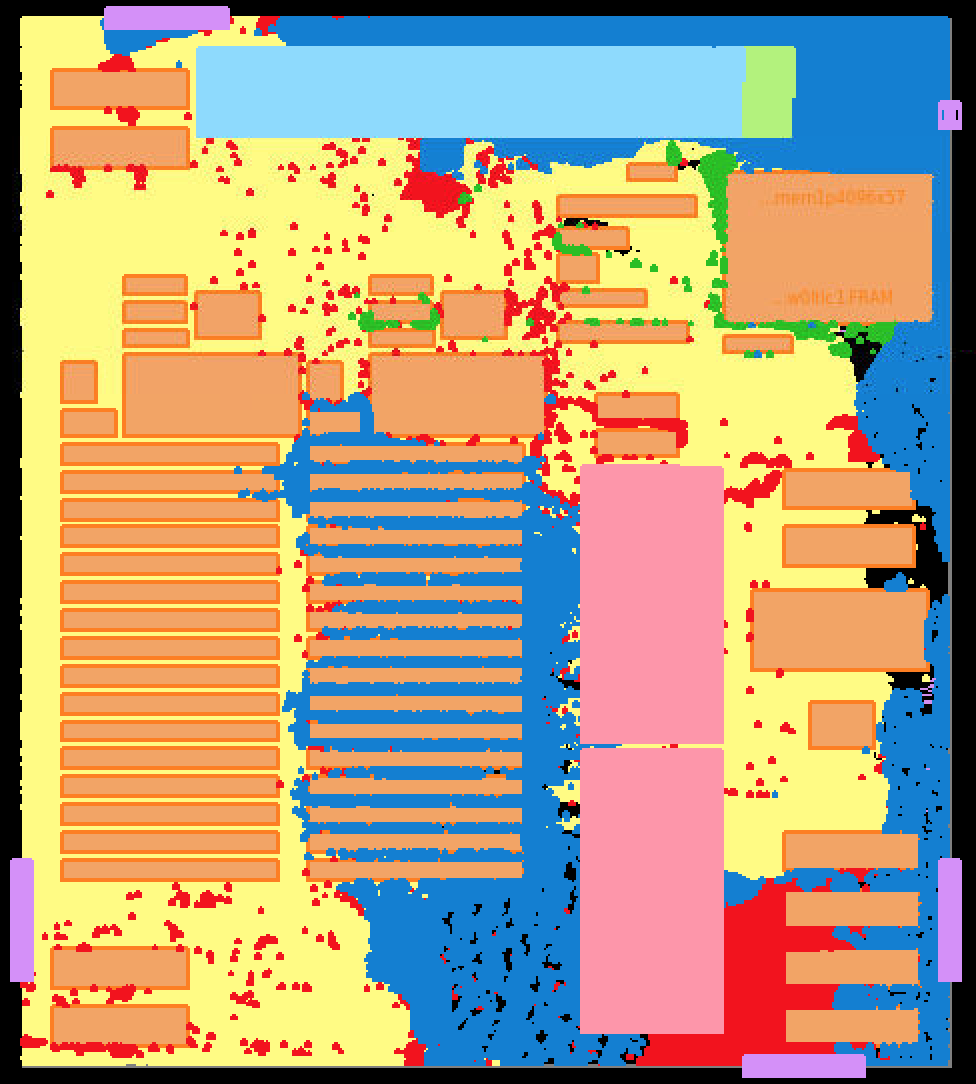
\includegraphics[width=0.95\textwidth]{ManagerLayout.png}
  \captionsetup{justification=centering, width=.8\linewidth}
  \caption{Manager}
  \label{fig:managerLayout}
\end{subfigure}%
\begin{subfigure}{.25\textwidth}
  \centering
  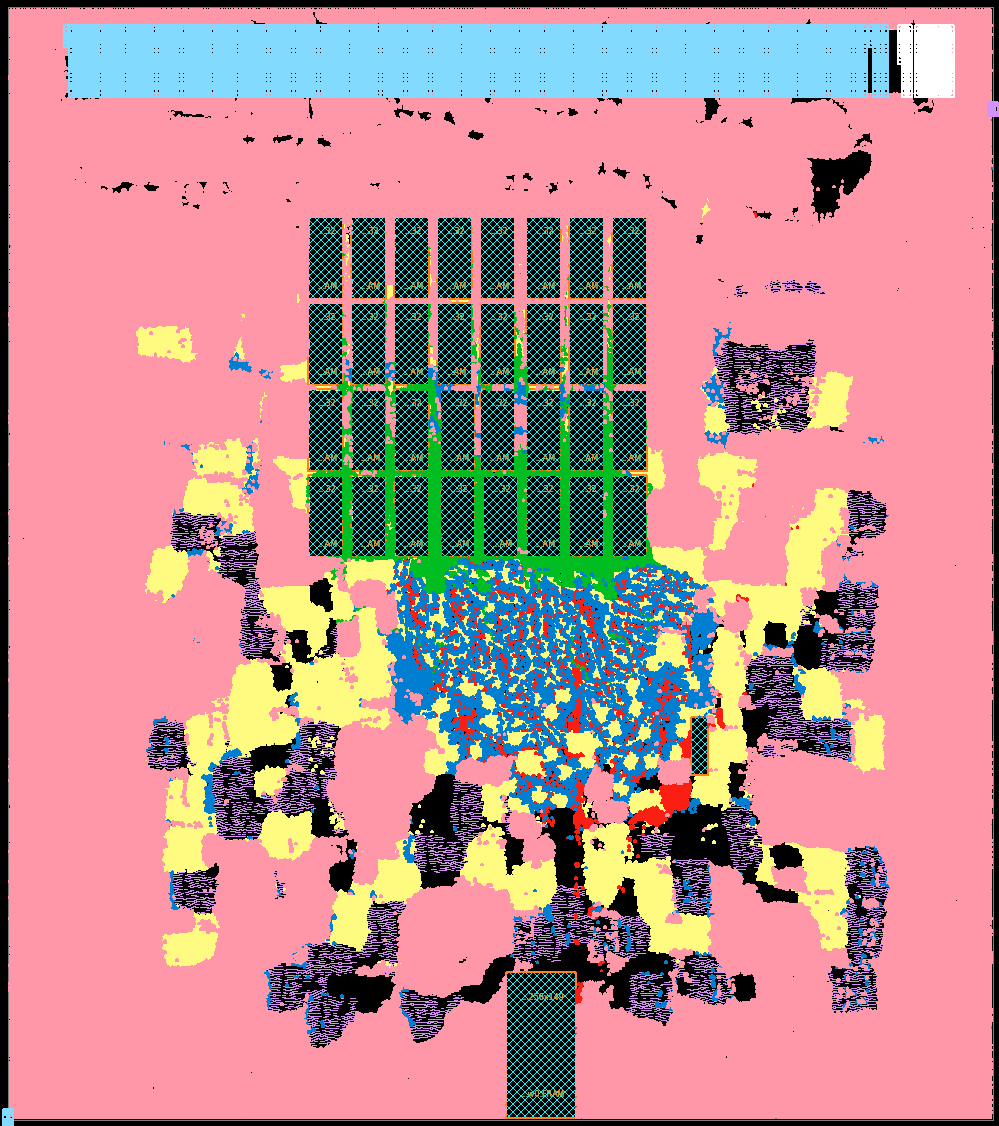
\includegraphics[width=0.95\textwidth]{PElayout.png}
  \captionsetup{justification=centering, width=.8\linewidth}
  \caption{PE}
  \label{fig:peLayout}
\end{subfigure}
\captionsetup{justification=centering, width=.9\linewidth}
\caption{Manager and PE Die layouts}
\label{fig:Manager and PE Die layouts}
\end{figure}


%%%%\begin{figure}[h]
%%%%\centering
%%%%\captionsetup{justification=centering}
%%%%    \begin{subtable}{.50\textwidth}
%%%%    %  \captionsetup{justification=centering, skip=-5pt}
%%%%      \centering
%%%%    %  \begin{center}
%%%%        % [lr] ~ left align col 0 and right align col 1
%%%%        % e.g. 4 columns could be lccr
%%%%        \resizebox{\textwidth}{!}{ % Scale table
%%%%        \begin{tabular}{r|ccc}
%%%%          \toprule
%%%%                         & \multicolumn{3}{c}{Technology} \\
%%%%                    Unit & \SI{130}{\nm} & \SI{65}{\nm} & \SI{45}{\nm}  \\
%%%%          \hline
%%%%          SIMD (32-lane) & 3200000 \\
%%%%                    DMA  &               & 368000  \\
%%%%      Memory Controller  &               & 294000  \\
%%%%                Control  &               & 1032000 \\
%%%%                   SRAM  &               & 740098  \\
%%%%                    FMA  &               &              & 405440 \\
%%%%          \bottomrule
%%%%        \end{tabular}
%%%%        }
%%%%      \captionsetup{justification=centering, skip=9pt}
%%%%      \vspace{-1mm}
%%%%      \caption{Original area estimates}
%%%%      \label{tab:areaEstimates}
%%%%    %  \end{center}
%%%%    \end{subtable}
%%%%    \hfill
%%%%    %\vfill
%%%%    \begin{subtable}{.45\textwidth}
%%%%    %  \captionsetup{justification=centering, skip=-5pt}
%%%%      \centering
%%%%    %  \begin{center}
%%%%        % [lr] ~ left align col 0 and right align col 1
%%%%        % e.g. 4 columns could be lccr
%%%%        \resizebox{\textwidth}{!}{%
%%%%        \begin{tabular}{r|cccc}
%%%%          \toprule
%%%%                            %& \multicolumn{4}{c}{Technology}   \\
%%%%                            &       &  Usable    &          &  \\  %\cline{1-1}
%%%%                            &       &   DRAM     & Expected &  \\  %\cline{1-1}
%%%%                            & Tech  & Bandwidth  &  Power   &  \\  %\cline{1-1}
%%%%          \hline  % instead of \midrule %midrule doesnt overlap with column lines
%%%%                  3D-System & 28    &       \SI[per-mode=symbol]{\sim 64}{\tera\bit\per\second}   &  73W   &  \\ %\cline{2-2}
%%%%                  NVidia    & 28    &  $\ll$\SI[per-mode=symbol]{1.28}{\tera\bit\per\second} &  100W  &  \\
%%%%                  TPU       & 28    &  $<$  \SI[per-mode=symbol]{224}{\giga\bit\per\second}  &  40W   &  \\
%%%%          \bottomrule
%%%%        \end{tabular}
%%%%        }
%%%%      \captionsetup{justification=centering, skip=9pt}
%%%%      \vspace{3mm}
%%%%      \caption{Scaling numbers (from \cite{schabel2014energy})}
%%%%      \label{tab:scalingNumbers}
%%%%    %  \end{center}
%%%%    \end{subtable}
%%%%\vspace{-2mm}
%%%%\caption{Original area estimates and scaling numbers}
%%%%\label{fig:areaAndScalingEstimates}
%%%%\end{figure}


% #######################################################################################################################################
% >>>>>>>>>>>>>>>>>>>>>>>>>>> Conclusions and Further Work <<<<<<<<<<<<<<<<<<<<<<
\section{Conclusions}
\label{sec:Conclusions}
There have been many attempts to accelerate ANNs. Many have shown excellent performance mainly when implementing CNNs. The improvement mostly comes from the ability to 
hold weights and/or AN activations in local SRAM and perform multiple operations whilst that data is held in local SRAM.
The ability to hold data in local SRAM is often due to pooling of batch requests or storing of CNN kernel weights or input Regions-of-Interest.
When considering applications where this local storage cannot be used effectively, all these implementation suffer large degradation in performance.


This work considers edge applications where a system is processing single requests into a disparate set of ANNs. The assumpiton is that local SRAM is no longer effective and performance is based on DRAM bandwidth.
This work considers 3DIC technology and the performance benefits it provides. In addition, a customized 3D-DRAM is proposed. The customized 3D-DRAM combined with a design based on custom instructions and operation descriptors
allows the system to achieve high levels of memory bandwidth efficiency.

There is no doubt CNN accelerators combined with batch processing achieve a performance that is difficult to better, but applying these systems to this works target application exposes the DRAM bandwidth limitations.

This work demonstrates a 3D-DRAM system that at the surface has a relatively low FLOPs, but the target applcation is memory bound and under these circumstances this work is potentially 10-100X better that existing ASIC/ASIPs or GPUs.

\section{Further Work}
\label{sec:Further Work}
This work does not put a high level of importance to the processing engine. The choice of using single-precision floating point format was in some part convenient. In fact, half-precision might have been a better choice especially as there
is a level of acceptance that lower precision is acceptable in ANN inference.
Therefore, further work should include :
\begin {outline}
  \1 Manager changes to support half-precision format
    \2 supports 16-bit FP would require additional muxing logic when directing words in the wide DRAM bus to execution lanes, but the bulk of the design should remain relatively intact.
  \1 Half-Precision PE
    \2 modifying the PE to support 16-bit FP would be relatively trivial
  \1 Additional PE pipelining
    \2 Adding layers of processing to the PE would effectively increase the operations per second
      \3 the PE area utilization is relatively low so it could support some additional pipelining
      \3 using a reduction array would effectively double the FLOPs
      \3 looking at storing weights and inputs for a pipelined PE would be required and the manager would likely be customized to the PE, but the belief is the Manager design and complexity should be similar
  \1 Systolic PE
    \2 systolic arrays have shown efficacy when used in server applications such as TPU, but its not clear how effective they would be in an edge application
      \3 consider how to effectively feed a systolic array PE
      \3 consider types of systolic array
      \3 consider situations such as multiple Managers feeding a single PE. For example, a systolic PE might use two managers to feed X and Y inputs of the array
 
\end{outline}


% Can use something like this to put references on a page
% by themselves when using endfloat and the captionsoff option.
\ifCLASSOPTIONcaptionsoff
  \newpage
\fi



% trigger a \newpage just before the given reference
% number - used to balance the columns on the last page
% adjust value as needed - may need to be readjusted if
% the document is modified later
%\IEEEtriggeratref{8}
% The "triggered" command can be changed if desired:
%\IEEEtriggercmd{\enlargethispage{-5in}}

% references section

% can use a bibliography generated by BibTeX as a .bbl file
% BibTeX documentation can be easily obtained at:
% http://mirror.ctan.org/biblio/bibtex/contrib/doc/
% The IEEEtran BibTeX style support page is at:
% http://www.michaelshell.org/tex/ieeetran/bibtex/
%\bibliographystyle{IEEEtran}
% argument is your BibTeX string definitions and bibliography database(s)
%\bibliography{IEEEabrv,../bib/Robot}
%
% <OR> manually copy in the resultant .bbl file
% set second argument of \begin to the number of references
% (used to reserve space for the reference number labels box)
\nocite{*}
\bibliographystyle{IEEEtran}
\bibliography{IEEEabrv,IEEE_jetcas}
%\bibliography{Robot}
%\begin{thebibliography}{1}
%\bibitem{IEEEhowto:kopka}
%H.~Kopka and P.~W. Daly, \emph{A Guide to \LaTeX}, 3rd~ed.\hskip 1em plus
%  0.5em minus 0.4em\relax Harlow, England: Addison-Wesley, 1999.
%\end{thebibliography}

% biography section
% 
% If you have an EPS/PDF photo (graphicx package needed) extra braces are
% needed around the contents of the optional argument to biography to prevent
% the LaTeX parser from getting confused when it sees the complicated
% \includegraphics command within an optional argument. (You could create
% your own custom macro containing the \includegraphics command to make things
% simpler here.)
%\begin{IEEEbiography}[{\includegraphics[width=1in,height=1.25in,clip,keepaspectratio]{mshell}}]{Michael Shell}
% or if you just want to reserve a space for a photo:
\begin{IEEEbiographynophoto}{Lee B. Baker}
received a B.S. degree in Electrical Engineering from Brighton Polytechnic, UK, an M.S. degree in Electrical Engineering from Villanova University, USA and an M.B.A. degree from North Carolina State University, USA in 1983, 1994 and 2009 respectively. He is currently pursuing the Ph.D. degree with the Electrical and Computer Engineering Department at North Carolina State University.
His current research interests include acceleration of artificial neural networks.
\end{IEEEbiographynophoto}
% if you will not have a photo at all:
\begin{IEEEbiographynophoto}{Paul Franzon}
is currently a Distinguished Alumni Professor of Electrical and Computer Engineering at North Carolina State University.  He earned his Ph.D. from the University of Adelaide, Adelaide, Australia in 1988.  He has also worked at AT\&T Bell Laboratories, DSTO Australia, Australia Telecom and three companies he cofounded, Communica, LightSpin Technologies and Polymer Braille Inc. His current interests center on the technology and design of complex microsystems incorporating VLSI, MEMS, advanced packaging and nano-electronics. He has lead several major efforts and published over 200 papers in these areas.  In 1993 he received an NSF Young Investigators Award, in 2001 was selected to join the NCSU Academy of Outstanding Teachers, in 2003, selected as a Distinguished Alumni Professor, and received the Alcoa Research Award in 2005.  He served with the Australian Army Reserve for 13 years as an Infantry Soldier and Officer.  He is a Fellow of the IEEE.
\end{IEEEbiographynophoto}

% You can push biographies down or up by placing
% a \vfill before or after them. The appropriate
% use of \vfill depends on what kind of text is
% on the last page and whether or not the columns
% are being equalized.

%\vfill

% Can be used to pull up biographies so that the bottom of the last one
% is flush with the other column.
%\enlargethispage{-5in}



% that's all folks
\end{document}


